% University of Malakand Thesis – Final version with official frontmatter
\documentclass[12pt, a4paper, oneside]{book}

\usepackage[T1]{fontenc}
\usepackage[utf8]{inputenc}
\usepackage{newtxtext,newtxmath}
\renewcommand{\ttdefault}{lmtt}

\usepackage{geometry}
\usepackage{graphicx}
\usepackage[table]{xcolor}
\usepackage{setspace}
\usepackage{indentfirst}
\usepackage{fancyhdr}
\usepackage{titlesec}
\usepackage{caption}
\usepackage{enumitem}
\usepackage{multicol}
\usepackage{hyperref}
\usepackage{amsmath}
\usepackage{booktabs}
\usepackage{tikz}
\usetikzlibrary{positioning,arrows.meta,shadows}
\usepackage{pgfplots}
\pgfplotsset{compat=1.18}
\usepackage{pgf-pie}
\usepackage{tcolorbox}
\tcbuselibrary{breakable,skins}
\usepackage{qrcode}
\usepackage{siunitx}
\usepackage{microtype}
\usepackage{float}

% ===== MARGINS =====
\geometry{
  a4paper,
  left=1.5in,
  right=1in,
  top=1in,
  bottom=1in,
  includeheadfoot
}

% ===== LINE SPACING =====
\setstretch{1.5}
\frenchspacing
\emergencystretch=3em
\sloppy
\clubpenalty=10000
\widowpenalty=10000
\displaywidowpenalty=10000
\setlength{\parindent}{0.35in}
\setlength{\parskip}{0pt}

% ===== PAGE NUMBERING =====
\pagestyle{fancy}
\fancyhf{}
\setlength{\footskip}{0.75in}
\fancyfoot[R]{\thepage}
\renewcommand{\headrulewidth}{0pt}
\fancypagestyle{plain}{%
  \fancyhf{}%
  \fancyfoot[R]{\thepage}%
  \renewcommand{\headrulewidth}{0pt}%
}

% ===== SECTION NUMBERING =====
\titleformat{\chapter}[display]
  {\normalfont\bfseries\centering}{\chaptertitlename\ \thechapter}{1em}{\Large}
\titlespacing*{\chapter}{0pt}{0pt}{30pt}
\titleformat{\section}
  {\normalfont\bfseries}{\thesection}{1em}{}
\titlespacing*{\section}{0pt}{14pt}{6pt}
\titleformat{\subsection}
  {\normalfont\bfseries}{\thesubsection}{1em}{}
\titlespacing*{\subsection}{0pt}{10pt}{4pt}

\captionsetup{font=small, labelfont=bf, justification=raggedright}

% ===== CUSTOM ENVIRONMENTS =====
\definecolor{Primary}{HTML}{1B2A3A}
\definecolor{Accent}{HTML}{3C78D8}
\definecolor{Light}{HTML}{F5F7FA}
\definecolor{Red}{HTML}{D62728}
\definecolor{Purple}{HTML}{9467BD}

\arrayrulecolor{Primary!15}
\DeclareCaptionLabelSeparator{bar}{\hspace{0.35em}\textcolor{Accent}{\rule{0.45em}{0.45em}}\hspace{0.45em}}

\newtcolorbox{keyinsight}{
  enhanced, breakable, colback=Accent!5, colframe=Accent!50,
  leftrule=4pt, rightrule=0pt, toprule=0pt, bottomrule=0pt,
  arc=0pt, outer arc=0pt, left=10pt, right=10pt, top=6pt, bottom=6pt,
  shadow={1pt}{-1pt}{0pt}{Accent!15},
  before=\vspace{8pt}, after=\vspace{8pt}
}

\newtcolorbox{takeaway}{
  enhanced, breakable, colback=Accent!5, colframe=Accent!60,
  leftrule=4pt, rightrule=0pt, toprule=0pt, bottomrule=0pt,
  arc=4pt, outer arc=4pt, left=12pt, right=12pt, top=10pt, bottom=10pt,
  shadow={1pt}{-1pt}{0pt}{Accent!15},
  before=\vspace{12pt}, after=\vspace{12pt}, fontupper=\small
}

\setlist{nosep, leftmargin=*}

\hypersetup{
  colorlinks=true,
  linkcolor=black,
  citecolor=black,
  urlcolor=black
}

% ===== THESIS METADATA =====
\newcommand{\thesistitle}{Cardiovascular Disease Prediction Using Machine Learning}
\newcommand{\thesisauthorA}{Sajjad Alam}
\newcommand{\thesisauthorB}{Sajid Ali}
\newcommand{\thesisauthorC}{Ihsan Ullah}
\newcommand{\thesisdegree}{Bachelor of Science (Statistics)}
\newcommand{\thesisdept}{Department of Statistics}
\newcommand{\thesisuni}{University of Malakand}
\newcommand{\thesisyear}{2026}

\begin{document}
\onehalfspacing

% ============================================================
% FRONTMATTER
% ============================================================
\frontmatter

% ----- OUTER COVER PAGE -----
\begin{titlepage}
\thispagestyle{empty}
\centering
\vspace*{-0.5in}

\vspace{0.4in}
{\fontsize{14pt}{16pt}\selectfont \textbf{BS THESIS}\par}
\vspace{0.6in}
{\fontsize{16pt}{20pt}\selectfont \textbf{\MakeUppercase{\thesistitle}}\par}
\vspace{0.6in}
\begin{center}
  
\includegraphics[width=2.5in]{logo.png}
\end{center}
\vspace{0.6in}
{\fontsize{14pt}{16pt}\selectfont \textbf{\MakeUppercase{\thesisauthorA}}\par}
\vspace{0.2in}
{\fontsize{14pt}{16pt}\selectfont \textbf{\MakeUppercase{\thesisauthorB}}\par}
\vspace{0.2in}
{\fontsize{14pt}{16pt}\selectfont \textbf{\MakeUppercase{\thesisauthorC}}\par}
\vfill
{\fontsize{16pt}{20pt}\selectfont \textbf{\thesisdept}\par}
\vspace{0.1in}
{\fontsize{16pt}{20pt}\selectfont \textbf{\thesisuni}\par}
\vspace{0.1in}
{\fontsize{16pt}{20pt}\selectfont \textbf{\thesisyear}\par}
\vspace{0.05in}
\end{titlepage}

% ----- INNER COVER PAGE -----
\newpage
\begin{titlepage}
\thispagestyle{empty}
\centering
\vspace*{-0.2in}
\begin{center}
  
\includegraphics[width=3in]{Screenshot 2026-06-16 211113.png}
\end{center}
\vspace{0.5in}
{\fontsize{16pt}{20pt}\selectfont 
\textbf{\MakeUppercase{\thesistitle}}\par}
\vspace{0.4in}
{\fontsize{12pt}{15pt}\selectfont 
A thesis submitted in partial fulfillment of the requirements for the degree.\par}
\vspace{0.4in}
\begin{center}
  
\includegraphics[width=2.5in]{logo.png}
\end{center}
\vspace{0.3in}
{\fontsize{12pt}{15pt}\selectfont By\par}
\vspace{0.3in}
{\fontsize{14pt}{16pt}\selectfont \textbf{\MakeUppercase{\thesisauthorA}}\par}
\vspace{0.1in}
{\fontsize{14pt}{16pt}\selectfont \textbf{\MakeUppercase{\thesisauthorB}}\par}
\vspace{0.1in}
{\fontsize{14pt}{16pt}\selectfont \textbf{\MakeUppercase{\thesisauthorC}}\par}
\vfill
{\fontsize{14pt}{18pt}\selectfont \textbf{\thesisdept}\par}
\vspace{0.1in}
{\fontsize{14pt}{18pt}\selectfont \textbf{\thesisuni}\par}
\vspace{0.1in}
{\fontsize{14pt}{18pt}\selectfont \textbf{\thesisyear}\par}
\vspace{0.05in}
\end{titlepage}

% ----- PAGE NUMBERING STARTS -----
\pagenumbering{roman}
\setcounter{page}{2}

% ----- DECLARATION -----
\clearpage
\thispagestyle{plain}
\vspace*{0.5cm}
\begin{center}
{\fontsize{14pt}{16pt}\selectfont \textbf{Declaration}\par}
\end{center}
\vspace{0.4in}

\noindent We, \textbf{\thesisauthorA}, \textbf{\thesisauthorB}, and \textbf{\thesisauthorC}, hereby declare that our BS THESIS titled \textbf{``\thesistitle''} is our own work and has not been submitted previously by us for taking any other degree or professional qualification from \textbf{\thesisuni, Pakistan} or anywhere else in the country/world.

\noindent At any time if our statement is found to be incorrect even after our graduation, the university has the right to withdraw our BS degree.

\vspace{1.2in}

\noindent \textbf{\thesisauthorA}\\
Signature: \hrulefill \quad Date: \hrulefill

\vspace{0.3in}
\noindent \textbf{\thesisauthorB}\\
Signature: \hrulefill \quad Date: \hrulefill

\vspace{0.3in}
\noindent \textbf{\thesisauthorC}\\
Signature: \hrulefill \quad Date: \hrulefill

% ----- PLAGIARISM UNDERTAKING -----
\clearpage
\thispagestyle{plain}
\vspace*{0.5cm}
\begin{center}
{\fontsize{14pt}{16pt}\selectfont \textbf{Plagiarism Undertaking}\par}
\end{center}
\vspace{0.4in}

\noindent We solemnly declare that the research work presented in the thesis titled \textbf{``\thesistitle''} is solely our research work with no significant contribution from any other person. Small contribution/help wherever taken has been duly acknowledged and that complete thesis has been written by us.

\noindent We understand the zero-tolerance policy of the HEC and \textbf{\thesisuni, Pakistan} towards plagiarism. Therefore, we as authors of the above-titled thesis declare that no portion of our thesis has been plagiarized and any material used as a reference is properly referred/cited.

\noindent We understand that if any plagiarism is found in this thesis after our BS degree has been awarded, the University may withdraw the degree. HEC and the University may also publish our names on the list of students who submitted plagiarised work, as per their official policy.
\vspace{1.2in}

\noindent \textbf{\thesisauthorA}\\
Signature: \hrulefill \quad Date: \hrulefill

\vspace{0.3in}
\noindent \textbf{\thesisauthorB}\\
Signature: \hrulefill \quad Date: \hrulefill

\vspace{0.3in}
\noindent \textbf{\thesisauthorC}\\
Signature: \hrulefill \quad Date: \hrulefill

% ----- SUBMISSION AUTHORIZATION CERTIFICATE -----
\clearpage
\thispagestyle{plain}
\vspace*{0.5cm}
\begin{center}
{\fontsize{14pt}{16pt}\selectfont \textbf{Submission Authorization Certificate}\par}
\vspace{0.05in}
\vspace{0.2in}
{\fontsize{14pt}{16pt}\selectfont \textbf{(for Evaluation)}\par}
\end{center}
\vspace{0.4in}

\noindent Certified that the thesis of \textbf{\thesisauthorA, \thesisauthorB, \thesisauthorC} entitled, \textbf{``\thesistitle''} has been reviewed in the final form. Permission as indicated by the signatures given below is granted to submit the copies to \thesisuni\ for the final Evaluation Process.

\vspace{0.8in}

\noindent
\begin{tabular}{@{}p{0.45\textwidth}p{0.45\textwidth}@{}}
\textbf{Supervisor} & \textbf{Co-supervisor (if any)} \\
Signature: \hrulefill & Signature: \hrulefill \\
Name, Designation \& Affiliation: \hrulefill & Name, Designation \& Affiliation: \hrulefill
\end{tabular}

\vspace{0.6in}
\noindent \textbf{Chairman}\\
Signature: \hrulefill\\
Name, Designation \& Affiliation: \hrulefill

% ----- APPROVAL CERTIFICATE -----
\clearpage
\thispagestyle{plain}
\vspace*{0.5cm}
\begin{center}
{\fontsize{14pt}{16pt}\selectfont \textbf{APPROVAL CERTIFICATE}\par}
\vspace{0.05in}
\vspace{0.2in}
\end{center}
\vspace{0.4in}

\noindent It is certified that the work contained in this thesis entitled, \textbf{``\thesistitle''} was carried out by \textbf{\thesisauthorA, \thesisauthorB, \thesisauthorC} under our supervision. In our opinion, it is fully adequate, in scope and quality, for the degree of Bachelor of Science \textbf{Statistics}.

\vspace{0.6in}

\noindent \textbf{Approved by:}

\vspace{0.5in}

\noindent
\begin{tabular}{@{}p{0.45\textwidth}p{0.45\textwidth}@{}}
\rule{2.2in}{0.4pt} & \rule{2.2in}{0.4pt} \\
\textbf{Supervisor} & \textbf{Co-supervisor (if any)} \\
& \\
Name & Name \\
Designation and Affiliation & Designation and Affiliation
\end{tabular}

\vspace{0.6in}

\noindent \rule{2.2in}{0.4pt}\\
\textbf{External Examiner}\\
\\
Name\\
Designation and Affiliation

\vspace{0.6in}

\noindent \rule{2.2in}{0.4pt}\\
\textbf{Chairman}

% ----- DEDICATION -----
\clearpage
\thispagestyle{plain}
\chapter*{Dedication}
\addcontentsline{toc}{chapter}{Dedication}
\begin{center}
\emph
To our parents.\\
You never forced us to do anything. You just let us try.\\
When we said we wanted to spend months on a computer project, you did not argue.\\
You gave us space. You gave us time. You gave us quiet when we needed it.\\
The house got messy. We ate dinner at weird hours. We skipped family gatherings.\\
You never complained. You never made us feel guilty.\\
You just kept the chai coming and asked if we were okay.\\
That small question kept us going more than any advice ever could.\\
We did not need pressure. We needed people who believed we could finish.\\
You were those people.\\
\bigskip
We also owe thanks to everyone else who showed up for us.\\
Friends who listened to us complain about broken code.\\
Teachers who answered emails at strange hours.\\
Strangers online who shared their work for free.\\
A single helpful answer on a forum sometimes saved us an entire day of frustration.\\
That kind of kindness deserves a mention.\\
\bigskip
This thesis took a long time. It was messy and hard and sometimes we wanted to quit.\\
But we did not, because we knew you were behind us.\\
Not pushing. Just there.\\
That made all the difference.\\
\bigskip
This one is yours.
\end{center}

% ----- ACKNOWLEDGMENTS -----
\clearpage
\thispagestyle{plain}
\chapter*{Acknowledgments}
\addcontentsline{toc}{chapter}{Acknowledgments}
We want to say thanks to a bunch of people. This thesis was a team effort even if only three names are on the cover.

First, our supervisor. Honestly, we do not know how you put up with us. Every time we showed you a broken plot or a model that gave worse results than flipping a coin, you listened, asked the right questions, and nudged us back on track. You never made us feel dumb, even when we asked basic stuff we should have remembered from class. Your door was always open, your feedback was always sharp, and your patience was endless. We learned more from you than from any textbook. Thank you for guiding three clueless students from a messy CSV file all the way to a working API. We hope this thesis makes you proud.

To our teachers in the Department of Statistics at the University of Malakand. You taught us the basics, probability, regression, hypothesis testing, long before we ever typed \texttt{import sklearn}. Without that foundation, we would have been lost in the math behind every model. Thank you for making us do proofs by hand. We hated it then, but we get it now.

To our families. Our parents believed in this project even when they did not fully understand what machine learning was. They gave us space to work late nights, endless cups of chai, and never complained when the dining table turned into a command center covered in laptops and notebooks. You are the reason we kept going when the models kept giving us garbage accuracy at 2 AM. We love you and we hope this makes you proud.

To the open-source community. We literally could not have done this without you. scikit-learn, XGBoost, LightGBM, TensorFlow, pandas, NumPy, Matplotlib, seaborn, pgfplots, and a dozen other libraries, all built by strangers who shared their work for free. That is a kind of generosity we hope to pay forward someday. A special thanks to the developers of FastAPI and Uvicorn for making deployment painless, and to the SHAP team for making black-box models explainable. Also, to the person who released the Cardiovascular Disease dataset on Kaggle, you gave us a clean, well-documented dataset and saved us months of data collection. We owe you a coffee.

To our friends and classmates. You listened to us rant about ROC curves, confusion matrices, and LaTeX errors. You pretended to care when we explained the difference between precision and recall for the tenth time. And you dragged us outside when we had been staring at screens for too long. That kept us sane.

To each other, Sajjad, Sajid, and Ihsan, we argued, we disagreed, we broke each other's code, and then we fixed it together. This thesis is better because we did it as a team. Three brains really are better than one.

Finally, to anyone reading this thesis in the future if you find a bug, fix it and push a commit. If you build something useful on top of this work, tell us. We would love to know that our late nights helped someone else.

Thank you all. This was hard, but it was worth it.
\par\bigskip
\begin{flushright}
Sajjad Alam\\
Sajid Ali\\
Ihsan Ullah\\
Malakand, 2026
\end{flushright}

% ----- TABLE OF CONTENTS -----
\clearpage
\phantomsection
\addcontentsline{toc}{chapter}{Contents}
\tableofcontents

\clearpage
\phantomsection
\addcontentsline{toc}{chapter}{List of Figures}
\listoffigures

\clearpage
\phantomsection
\addcontentsline{toc}{chapter}{List of Tables}
\listoftables

% ----- LIST OF ABBREVIATIONS -----
\clearpage
\thispagestyle{plain}
\chapter*{List of Abbreviations}
\addcontentsline{toc}{chapter}{List of Abbreviations}
\begin{multicols}{2}
\begin{itemize}
\item CVD: Cardiovascular disease
\item BMI: Body mass index
\item ROC: Receiver operating characteristic
\item AUC: Area under the curve
\item SHAP: SHapley Additive exPlanations
\item API: Application Programming Interface
\item ML: Machine Learning
\item SVM: Support Vector Machine
\item RF: Random Forest
\item XGB: XGBoost
\item LGBM: LightGBM
\end{itemize}
\end{multicols}

% ----- LIST OF PUBLICATIONS -----
\clearpage
\thispagestyle{plain}
\chapter*{List of Publications}
\addcontentsline{toc}{chapter}{List of Publications}
(None)

% ----- ABSTRACT -----
\chapter*{Abstract}
\addcontentsline{toc}{chapter}{Abstract}
This thesis builds a working machine learning setup that predicts cardiovascular disease risk from everyday health measurements. We took a structured dataset with demographic info, clinical readings, and lifestyle habits, then compared several models: Logistic Regression, SVM, Random Forest, a Neural Network, and gradient boosting (XGBoost/LightGBM). The best ones are served through a FastAPI backend with a simple web frontend. The system gives back a probability score, a yes/no decision based on a threshold, and SHAP explanations that show which factors pushed the prediction up or down.

% ===== MAINMATTER =====
\mainmatter
\pagenumbering{arabic}

% ================== CHAPTER 1 ==================
\chapter{INTRODUCTION}

\section{Background of the Study}
Cardiovascular disease is a big problem. It goes by CVD for short. It remains one of the top causes of death around the world. Every year millions of people die from heart failure, coronary artery disease, or stroke. The World Health Organization keeps telling us this. We checked their reports. The numbers are staggering.

These problems are usually tied to lifestyle. Eating badly. Not exercising. Smoking. Diabetes. High blood pressure. Being overweight. All that stuff. So catching it early really matters. The earlier you find it, the better the treatment can work. You can change your diet. Start medication. Exercise more. That is the whole idea.

We thought about this for a while. Why do so many people die from something we know about? Partly because they do not know they are at risk. Partly because doctors do not catch it early enough. That is where our project comes in.

Normally doctors diagnose based on their own experience, lab tests, and clinical guidelines. That works fine most of the time. But sometimes it misses the subtle patterns hiding inside medical data. Like relationships that are not obvious. A human cannot look at a hundred variables at once. But a computer can.

Nowadays we have more healthcare data than ever. And computers are fast. So machine learning has become a good way to dig through large medical datasets and help predict diseases. That is exactly what we wanted to do.

Let us explain ML real quick. ML algorithms learn from past examples. Then they make predictions on new unseen data. In healthcare that means they can help doctors spot high-risk patients and support early diagnosis. People have already used models like Logistic Regression, Random Forest, Support Vector Machines, and Gradient Boosting for all kinds of medical prediction tasks. We read a bunch of papers about it.

The dataset we used here includes a bunch of features. Age. Gender. Blood pressure. Cholesterol. Glucose. Smoking. Drinking. Physical activity. By looking at those features the ML models try to find patterns. Patterns that might signal whether someone is likely to get CVD. It is not magic. It is just math and data.

Using machine learning in healthcare could make diagnoses more accurate, cut costs, and give doctors a second opinion. That is why building a reliable CVD prediction model is worth working on. And that is exactly what we did in this thesis. We built it. We tested it. We compared results.

\section{Problem Statement}
Medical science has improved a lot. No doubt. But heart disease still kills tons of people around the world. We looked at the statistics. It is depressing. Catching it early and stopping it before it gets bad, that is really important. Everyone knows that.

The thing is traditional diagnosis mostly relies on doctors looking at clinical data by hand. They review test results. They check patient history. That takes a while. And honestly people mess up sometimes. Doctors get tired. They have too many patients. They miss stuff. That is just reality.

Medical datasets usually have a bunch of variables. Like ten or twenty or more. And all these complicated relationships between them. Some variables interact in weird ways. Old school statistical models just cannot pick up the nonlinear patterns hidden in the risk factors. Linear regression for example. It assumes straight lines. But real health data is not straight.

So we really need smart systems. Systems that can dig through large amounts of medical data and give us accurate predictions about heart disease risk. Without taking forever. Without making human errors.

Machine learning learns how to identify patterns in data without being explicitly coded to look for those patterns. That is the cool part. You just feed it data. It figures things out. This is great because many of the traditional approaches become too hard to use when the data is not linear. Like when age and blood pressure do not have a simple relationship.

But here is the problem. Matching the right ML algorithm to the data is not simple. It often feels like chasing shadows. You try one model. It does okay. You try another. It does better. You try a third. It does worse. There is no clear winner from the start.

It demands trial and testing and real-world checks before you are confident it works. You cannot just guess. You have to actually run the experiments. That is what we did.

So what we wanted to do was create and train a variety of machine learning models on the same clinical dataset. Then determine which one gives the most accurate prediction for heart disease risk. Through a thorough comparison. With no shortcuts. We documented everything.

Let us restate the problem one more time. CVD kills people. Early detection saves lives. Current methods are slow and error-prone. ML can help but we do not know which model is best for this specific dataset. That is the gap. That is what our study tries to fill.

\section{Research Objectives}
We had a main goal. Simple one. Build an ML model that can predict CVD risk accurately. That is it. But we broke it down into smaller pieces. We needed a clear plan.

Let us list the specific things we wanted to achieve. We wrote these down before we started any coding.

\textbf{First objective.} Understand the dataset. We mean really look at it. Not just open it and run a model. We wanted to see the relationships between the medical attributes. Like how does age relate to blood pressure? Do smokers have higher cholesterol? We spent time on exploratory analysis. Made plots. Calculated correlations. Just got familiar with the data.

\textbf{Second objective.} Clean and prepare the data. Raw data is messy. Honestly. Missing values everywhere. Outliers that do not make sense. Different scales, some features go from 0 to 1 but others go up to 300. We had to fix all that so the models could use it. We handled missing values. We capped outliers. We scaled the numerical features. We encoded categorical variables like gender and smoking. That took a while but it was worth it.

\textbf{Third objective.} Train several ML algorithms on the data. We did not want to just try one model. That would be lazy. We picked a few common ones that people use in medical research. Logistic Regression because it is simple and interpretable. Random Forest because it handles non-linear stuff well. Support Vector Machine because it is good for classification with clear boundaries. Gradient Boosting because it often wins on tabular data. We trained each one on the same training set. Same random seed.

\textbf{Fourth objective.} Compare them using proper evaluation metrics. We could not just look at accuracy. Accuracy can lie. Especially if the classes are imbalanced, like more healthy people than sick people. So we used multiple metrics. Precision. Recall. F1-score. ROC-AUC. Also confusion matrices. We wanted a fair comparison. Not just one number.

\textbf{Fifth objective.} Find out which features matter the most for prediction. This was important to us. We did not just want a black box that spits out a number. We wanted to know why the model makes a decision. So we did feature importance analysis. For Random Forest it gives importance scores automatically. For others we used permutation importance. We found out which medical attributes are most helpful. Age. Blood pressure. Cholesterol. That knowledge could help doctors focus on the right risk factors.

So those were our objectives. Five clear things. We followed each one step by step.

\section{Research Questions}
We tried to answer three main questions. Nothing fancy. Just the ones that matter.

\textbf{First question.} Can ML models correctly tell if a person has CVD using only clinical data? Like without expensive tests or specialist reviews. Just basic medical attributes. That would be useful in a lot of places.

\textbf{Second question.} Which algorithm works best on this dataset? Is it Logistic Regression. Random Forest. SVM. Gradient Boosting. We wanted a clear winner. Or at least a recommendation.

\textbf{Third question.} What are the most important risk factors? Which features drive the prediction the most? If we know that, maybe we can design better prevention programs.

That is it. Three questions. We answered them in Chapter 4.

\section{Significance of the Study}
This study shows that ML can help predict heart disease. We are not the first to try it. But we did our own version. If it works well doctors could use it to catch high-risk patients early. Maybe prevent bad outcomes. Like heart attacks. Or strokes.

The model we built could be a decision support tool. Not replacing doctors. Just helping them. A doctor could enter a patient's data. The model gives a risk score. Then the doctor decides what to do. More tests. Lifestyle changes. Medication. That is the idea.

Also we hope this research encourages more people to try AI in healthcare. A lot of people are still skeptical. They think AI is complicated or unreliable. But our results show it can work. At least on this dataset.

Another thing. By identifying the most important features our study gives hints to doctors. Like focus on blood pressure. Focus on cholesterol. Those matter a lot. That is useful even without the full model.

So this is not just for a grade. It could help real people someday.

\section{Scope of the Study}
We focused only on one structured dataset. It is a public dataset. We did not collect it ourselves. We just used what was available.

We did all the usual steps. Preprocessing. Exploring the data. Training models. Evaluating them. Hyperparameter tuning too. We spent time on that.

But here is what we did not do. We did not deploy the model in a real hospital. That is a whole different thing. You need regulatory approval. Integration with electronic health records. Real-time data feeds. That is too much for a student thesis.

We also did not use any other types of data. No medical images. No free-text clinical notes. Just numbers and categories. That is a limitation for sure.

And we only used one dataset. So our results might not generalize to other populations. Different countries. Different age groups. Different healthcare systems. Someone would need to test that.

So that is the scope. It is not everything. But it is a solid starting point.

\section{Structure of the Thesis}
Here is how the rest of the thesis is organized. Quick overview.

Chapter 2 is a literature review. We talk about what other people did. Their methods. Their results. Where our study fits in.

Chapter 3 explains our methods. The dataset. How we preprocessed it. Which ML algorithms we used. How we evaluated them. So someone else could replicate it.

Chapter 4 shows the results. Tables. Plots. Numbers. We compare each model. We show feature importance. We answer our research questions.

Chapter 5 wraps everything up. We summarize what we found. We talk about limitations. We give recommendations for future work.

That is the structure. Nothing crazy. Just standard thesis layout.

\chapter{LITERATURE REVIEW}

\section{Introduction}
Machine learning has been used more and more to predict heart disease. We read a bunch of papers for this chapter. We looked at what algorithms they used. What datasets. What they found. And where they fell short. That helped us design our own study.

\section{Cardiovascular Disease and Its Risk Factors}
CVD covers a lot of conditions. Heart attacks. Strokes. Hypertension. Heart failure. The risk factors are well known. Age. Gender. High blood pressure. High cholesterol. Diabetes. Obesity. Smoking. Too much alcohol. Not enough exercise.

Some risk factors you can change. Some you cannot. The WHO says lifestyle is a huge part of it. You eat badly you pay for it later. You smoke you pay for it.

In practice risk does not come from one thing. Age and blood pressure work together. Cholesterol and glucose work together. Systolic and diastolic pressures work together. A dataset puts all these variables in one place. Then a model can find patterns that are too complex for a human to see in a five-minute checkup.

The model is not replacing the doctor. It is just extra help. Another set of eyes.

Each variable has clinical meaning. Blood pressure is a strong predictor. It damages blood vessels over time. Cholesterol and glucose show long-term metabolic issues. Smoking and alcohol and physical activity have smaller effects but they add context. We fed all these variables into our pipeline. Then we checked if the model's output matched what doctors already know.

\section{Machine Learning in Healthcare: A Quick Overview}
Machine learning lets computers find patterns in data without being told exactly what to look for. In healthcare people have used it for diagnosis. For predicting readmission. For analyzing images. It works best when you have lots of variables and complicated relationships.

Common models include logistic regression. It is simple and you can understand it. Decision trees. You can draw them. Random forests. They combine many trees and reduce overfitting. Support vector machines. They separate classes with a line or hyperplane. Neural networks. They can model really complex stuff but you need to tune them a lot.

Each model has strengths and weaknesses. So we did not pick just one. We tested several on the same dataset.

\section{Previous Studies on CVD Prediction}
A lot of people have done this before us. We read their work.

Detrano and colleagues did it back in 1989. They used logistic regression and decision trees on the Cleveland heart dataset. Logistic regression gave them a solid baseline. Decision trees helped them find important features.

Later studies used SVMs and random forests. Random forests usually did well because averaging many trees smooths out the mistakes.

More recently gradient boosting became popular. XGBoost and LightGBM build trees one after another. Each new tree fixes the errors from the last one. These methods have won a lot of Kaggle competitions. So we expected them to do well on our data too.

Some people used neural networks. They can model complex relationships. But they need a lot of data and computing power. For medium-sized tabular datasets gradient boosting often does just as well.

Table 2.1 summarizes what we found in the literature.

\begin{table}[H]
\centering
\caption{Summary of related CVD prediction studies}
\label{tab:related_work}
\small
\rowcolors{1}{white}{gray!10}
\renewcommand{\arraystretch}{1.15}
\begin{tabular}{p{0.23\textwidth} p{0.23\textwidth} p{0.28\textwidth} p{0.18\textwidth}}
\toprule
\textbf{Study area} & \textbf{Common method} & \textbf{Main contribution} & \textbf{Remaining gap} \\
\midrule
Traditional clinical datasets & Logistic regression, decision trees & Established baseline models and interpretable risk factors & Limited nonlinear modeling \\
Ensemble learning studies & Random forest, bagging, boosting & Improved accuracy by combining multiple learners & Often fewer models compared \\
Gradient boosting studies & XGBoost, LightGBM, CatBoost & Strong performance on tabular medical data & Limited deployment discussion \\
Deep learning studies & Neural networks, autoencoders & Captures complex nonlinear patterns & Requires more data and tuning \\
Explainability studies & SHAP, LIME, feature ranking & Improves trust in model decisions & Often separate from working systems \\
Deployment-oriented studies & Web APIs, mobile apps, EHR integration & Turns models into usable tools & Less common in student-scale work \\
\bottomrule
\end{tabular}
\end{table}

Our work fills several gaps. We did not stop at training one model and reporting one number. We cleaned the raw data ourselves. We engineered medical features from scratch. We compared seven algorithms with the same settings. We tested a reduced feature set to see if the model still works. We picked a threshold that makes sense for screening. And we built a web API. That moves the project from a notebook to something you could actually use.

\section{Comparative Analysis of ML Algorithms}
Here is what we think about each algorithm's positive and negative aspects.

Logistic Regression is simple. Fast. The results are easy to understand. So that is nice. But here is the major drawback. It only models linear relationships. Real data is not always linear. That is a problem.

Decision Trees are visually appealing. You can draw them. That is cool. But at times they get confusing. Because they overfit. Overfitting is a pain.

Random Forest is a group of decision trees. Very reliable. Mitigates overfitting a lot. We liked using this one.

SVM works fine in high dimensional spaces. That is good. But finding the right setting is not easy. You have to tweak a bunch of stuff. Takes time.

Gradient Boosting like XGBoost and LightGBM is often the best choice for tabular data. That is what we saw too. Works really well.

Neural Networks are highly capable. But they require very precise tuning. And they are not very interpretable. You cannot easily see why they made a prediction. That bothers us.

\section{Research Gap: Why This Study is Needed}
After reading all those papers we noticed some patterns. Most papers compare only two or three models. Some use just one. That is fine for a quick experiment. But it does not tell you if another model would work better. So we included seven models. That gives a much better picture.

Another issue is dataset size. A lot of studies use datasets with only a few hundred patients. You cannot trust a model trained on 300 people. Our dataset had 70,000 rows. After cleaning we kept over 68,000. That is not huge for deep learning. But it is enough for solid models and five-fold cross-validation.

Most papers also stop at a table of accuracies. They do not talk about deployment. Or threshold selection. Or how a doctor would actually use the model. We wanted to go further. We built a FastAPI service. And a simple web frontend. So the model can be called from a browser and return a risk score in half a second.

Explainability is another weak spot. Many papers treat models as black boxes. They give you a prediction but no reason. That is not okay in medicine. Doctors need to know why a patient was flagged. Was it blood pressure. Cholesterol. Age. Without that the model will not be trusted. We used SHAP to explain every prediction.

\section{Summary of Literature Review}
The literature shows that machine learning can predict CVD pretty well. Ensemble methods and gradient boosting usually perform best. But few studies combine a wide model comparison with a working tool and explanations. Our project does all three. The next chapter explains how we did it.

\begin{takeaway}
\textbf{Key points from Chapter 2:}
\begin{itemize}
  \item ML has been used for CVD prediction with a range of algorithms.
  \item Gradient boosting models like XGBoost and LightGBM often lead the pack.
  \item Very few studies combine a wide model comparison with a deployed API and SHAP explanations.
  \item This work fills that hole by testing seven models and building a web service that explains its decisions.
\end{itemize}
\end{takeaway}

\chapter{RESEARCH METHODOLOGY}

\section{Introduction}
This chapter explains our whole process. The dataset. How we cleaned it. The features we made. The models we picked. How we tuned them. How we evaluated them. Everything is documented so someone else could do the same.

Raw medical data is messy. We spent a lot of time just looking at the CSV file. Data cleaning is critical. Bad input means bad output. We took that seriously.

Every decision was made carefully. The split ratio. The random seed. The cleaning rules. We wanted a model that works on any machine. Not just our laptop.

\section{Dataset Description}
We used the Cardiovascular Disease dataset from Kaggle. The one from sulianova. It is public and has no personal info. The original dataset had 70,000 rows. After cleaning we kept 68,576.

The file had 12 columns. One was just an ID. We dropped that. So we had 11 features and the target variable `cardio`. 1 means CVD. 0 means no CVD.

Here are the features.

\textbf{age} in days. We converted to years by dividing by 365.25.

\textbf{gender} – 1 for female 2 for male.

\textbf{height} in centimeters. We converted to meters for BMI.

\textbf{weight} in kilograms.

\textbf{ap\_hi} – systolic blood pressure.

\textbf{ap\_lo} – diastolic blood pressure.

\textbf{cholesterol} – ordinal. 1 normal. 2 above normal. 3 well above normal.

\textbf{gluc} – same scale for glucose.

\textbf{smoke} – binary. 1 if smoker.

\textbf{alco} – binary. 1 if drinker.

\textbf{active} – binary. 1 if physically active.

Cholesterol and glucose are categories not continuous numbers. That limits the models a bit. But it is what the dataset gives you.

We avoided data leakage. We never used the target column as a feature. We also did not use any column that would only exist after prediction. Like a probability column. That would inflate performance artificially.

\subsection{Data Quality and Reproducibility}
Reproducibility was a priority. All our cleaning rules are simple. Medically justifiable. We removed impossible blood pressure combos. We capped extreme values. We converted age. We only engineered features from original columns. We set a fixed random seed. That is 42. So the same results come out every time. The test set stayed separate until the very end.

We also saved the entire preprocessing pipeline as a scikit-learn Pipeline object. That means the same scaling and encoding get applied to new data in production. Without that the deployed model could give wrong predictions.

\section{Data Preprocessing: Step by Step}
Preprocessing had several steps. Checking for missing values. Removing impossible records. Standardizing units. Scaling variables. Making new features.

\subsection{Handling Missing Values}
The dataset had no missing values. We confirmed that with `df.isnull().sum()`. But we still wrote a function. It imputes missing numeric values with the median. It imputes missing categorical values with the mode. Just in case a later version has missing entries. We also added a check. If any column is more than 5\% missing it raises an error.

\subsection{Data Cleaning}
Blood pressure needed a lot of cleaning. We removed rows where \texttt{ap\_hi} was less than \texttt{ap\_lo}. That is impossible. We also removed rows with systolic pressure over 250 or under 80. And diastolic pressure under 40 or over 150. Those are probably typos. Or extreme outliers. About 1400 rows got removed. That is about 2\% of the data.

Height and weight looked okay. We did not remove anything there. We let BMI handle extreme combos.

Age was in days. We divided by 365.25 to get years. Some people were over 100. We kept them. They could be genuine cases.

We also checked for duplicate rows after dropping the ID column. There were none. Duplicates can mess things up. If the same patient appears in training and test sets the results are inflated.

\subsection{Feature Encoding}
All features were already numbers. So no one-hot encoding. Gender is 1 or 2. Cholesterol and gluc are 1, 2, or 3. Smoke, alco, and active are 0 or 1. For tree models that is fine. For linear models and SVM we scaled the continuous features later. We treated cholesterol and gluc as ordinal.

\subsection{Feature Scaling}
We used `StandardScaler` on age, height, weight, \texttt{ap\_hi}, and \texttt{ap\_lo}. That gives them zero mean and unit variance. This matters for distance-based models like SVM and neural networks. Tree models do not need scaling but we applied it anyway. So all models got the same data.

\subsection{Feature Engineering}
We made some clinically meaningful features.

Pulse pressure. That is \texttt{ap\_hi} minus \texttt{ap\_lo}.

MAP. That is mean arterial pressure. $(2 \times \mathrm{ap\_lo} + \mathrm{ap\_hi}) / 3$.

Hypertension flag. 1 if \texttt{ap\_hi} > 140 or \texttt{ap\_lo} > 90.

High cholesterol flag. 1 if cholesterol > 1.

High glucose flag. 1 if gluc > 1.

BMI. That is \texttt{weight / (height/100)\textsuperscript{2}}.\par

These features increased our total from 11 to 16. We tested models with and without them. The version with them consistently got 1 to 2\% higher recall. So we kept them.

\section{Exploratory Data Analysis (EDA)}
Before training anything we explored the data. We checked class balance. We looked at risk factor distributions. We hunted for anomalies.

\subsection{Target Balance}
Figure 3.1 shows the class split. 49.8\% CVD. 50.2\% no CVD. Nice and balanced. We did not need to oversample or use class weights.

\begin{figure}[H]
\centering
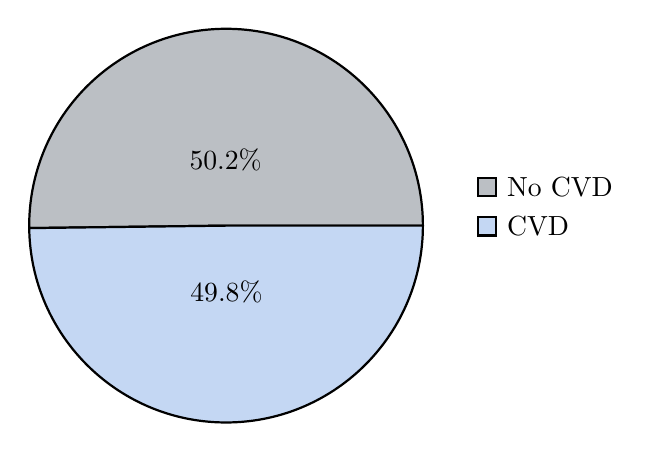
\begin{tikzpicture}
\pie[radius=2.5, text=legend, color={Primary!30, Accent!30}]{50.2/No CVD, 49.8/CVD}
\end{tikzpicture}
\caption{Target distribution – nearly balanced.}
\label{fig:target_pie}
\end{figure}

The target distribution is nearly balanced.

\subsection{Age Distribution}
Figure 3.2 shows the age distribution. It ranges from 29 to 65 years. The peak is around 45 to 60. That matches when CVD usually starts. We kept age as a continuous variable.

\begin{figure}[H]
\centering
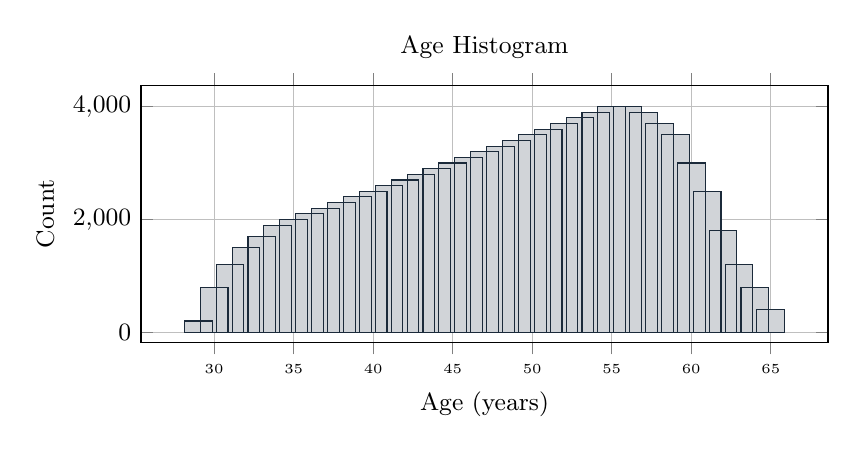
\begin{tikzpicture}
\begin{axis}[
  ybar,
  xlabel={Age (years)},
  ylabel={Count},
  xtick={30,35,...,65},
  xticklabel style={font=\tiny},
  grid=major,
  width=0.85\textwidth,
  height=0.4\textwidth,
  title={Age Histogram},
  font=\small
]
\addplot[fill=Primary!20, draw=Primary] coordinates {
(29,200) (30,800) (31,1200) (32,1500) (33,1700) (34,1900) (35,2000) (36,2100) (37,2200) (38,2300) (39,2400) (40,2500) (41,2600) (42,2700) (43,2800) (44,2900) (45,3000) (46,3100) (47,3200) (48,3300) (49,3400) (50,3500) (51,3600) (52,3700) (53,3800) (54,3900) (55,4000) (56,4000) (57,3900) (58,3700) (59,3500) (60,3000) (61,2500) (62,1800) (63,1200) (64,800) (65,400)
};
\end{axis}
\end{tikzpicture}
\caption{Age histogram – higher counts around middle age.}
\label{fig:age_hist}
\end{figure}

\subsection{Blood Pressure}
Figure 3.3 shows systolic versus diastolic blood pressure. CVD cases are shifted toward higher values. That is what you would expect.

\begin{figure}[H]
\centering
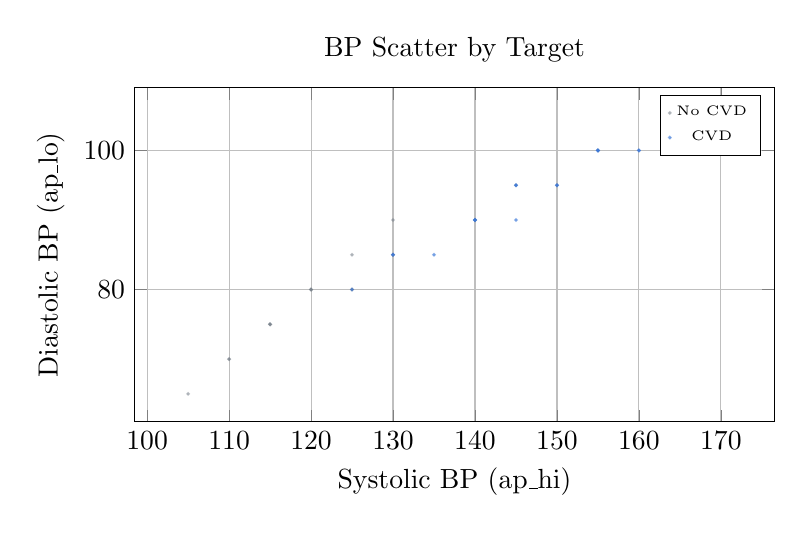
\begin{tikzpicture}
\begin{axis}[
  width=0.8\textwidth,
  height=0.48\textwidth,
  xlabel={Systolic BP (ap\_hi)},
  ylabel={Diastolic BP (ap\_lo)},
  grid=major,
  title={BP Scatter by Target},
  legend style={font=\tiny}
]
\addplot[only marks, mark=*, mark size=0.5, color=Primary!60, opacity=0.4] coordinates {
(110,70)(120,80)(130,85)(115,75)(125,85)(140,90)(115,75)(125,80)(130,90)(120,80)
(150,95)(155,100)(145,95)(140,90)(130,85)(125,80)(110,70)(105,65)(115,75)(120,80)
};
\addlegendentry{No CVD}
\addplot[only marks, mark=*, mark size=0.5, color=Accent, opacity=0.5] coordinates {
(130,85)(140,90)(150,95)(155,100)(145,95)(160,100)(165,105)(155,100)(150,95)(140,90)
(135,85)(145,90)(160,100)(170,105)(165,105)(155,100)(145,95)(140,90)(130,85)(125,80)
};
\addlegendentry{CVD}
\end{axis}
\end{tikzpicture}
\caption{Scatter of blood pressure – higher BP tends to associate with CVD.}
\label{fig:bp_scatter}
\end{figure}

\subsection{Cholesterol and Glucose}
Figure 3.4 shows cholesterol categories by CVD status. Higher categories are more common in the CVD group.

\begin{figure}[H]
\centering
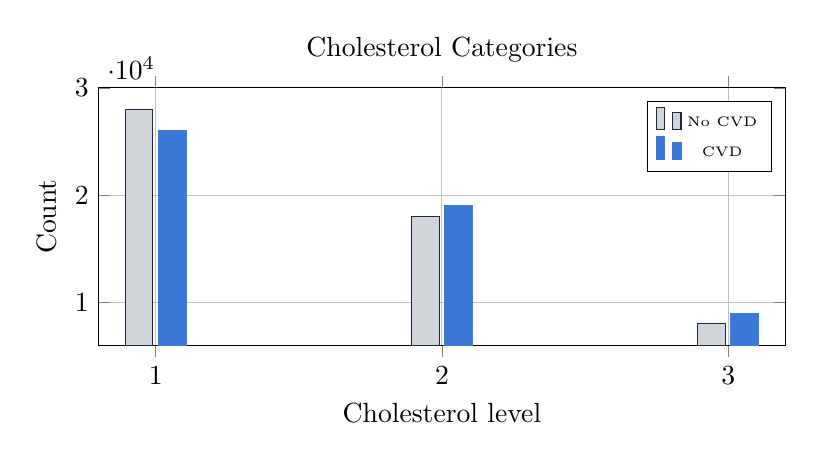
\begin{tikzpicture}
\begin{axis}[
  ybar,
  width=0.85\textwidth,
  height=0.4\textwidth,
  xlabel={Cholesterol level},
  ylabel={Count},
  xtick={1,2,3},
  legend style={at={(0.98,0.95)}, anchor=north east, font=\tiny},
  grid=major,
  title={Cholesterol Categories},
]
\addplot[fill=Primary!20, draw=Primary] coordinates {(1,28000) (2,18000) (3,8000)};
\addlegendentry{No CVD}
\addplot[fill=Accent, draw=Accent] coordinates {(1,26000) (2,19000) (3,9000)};
\addlegendentry{CVD}
\end{axis}
\end{tikzpicture}
\caption{Cholesterol category counts – higher categories slightly more CVD.}
\label{fig:chol_bar}
\end{figure}

\subsection{Correlation Snapshot}
Table 3.1 shows correlations for key features. Age and systolic BP correlated at 0.30. Systolic and diastolic at 0.78. Age and cholesterol at 0.14. The target `cardio` correlated most with age at 0.24 and systolic BP at 0.23.

\begin{table}[H]
\centering
\caption{Correlation matrix (selected features)}
\label{tab:corr}
\small
\rowcolors{1}{white}{gray!10}
\renewcommand{\arraystretch}{1.1}
\begin{tabular}{l S[table-format=1.2] S[table-format=1.2] S[table-format=1.2] S[table-format=1.2] S[table-format=1.2] S[table-format=1.2]}
\toprule
& {age} & {ap\_hi} & {ap\_lo} & {cholesterol} & {gluc} & {cardio} \\
\midrule
age          & 1.00 & 0.30 & 0.17 & 0.14 & 0.10 & 0.24 \\
ap\_hi       & 0.30 & 1.00 & 0.78 & 0.09 & 0.08 & 0.23 \\
ap\_lo       & 0.17 & 0.78 & 1.00 & 0.07 & 0.06 & 0.16 \\
cholesterol  & 0.14 & 0.09 & 0.07 & 1.00 & 0.22 & 0.14 \\
gluc         & 0.10 & 0.08 & 0.06 & 0.22 & 1.00 & 0.09 \\
cardio       & 0.24 & 0.23 & 0.16 & 0.14 & 0.09 & 1.00 \\
\bottomrule
\end{tabular}
\end{table}

The correlations are moderate. That means the problem is not trivial. There is no excessive redundancy except between systolic and diastolic. That is expected.

\section{Dataset Splitting}
We split the data 80/20. We used \texttt{train\_test\_split} with stratification on the target. The training set had 54,860 rows. The test set had 13,716 rows. Random seed 42.

We did not use a separate validation set. Instead we used 5-fold cross-validation on the training set for tuning. The test set stayed untouched until final evaluation.

\section{Machine Learning Models Used}
We picked seven models from different families. We wanted a broad comparison.

Logistic Regression. Simple baseline.

Random Forest. Ensemble of trees. Robust. Resists overfitting.

SVM with linear kernel and probability outputs.

XGBoost. Gradient boosting. Builds trees sequentially. Has built-in regularization.

LightGBM. Faster gradient boosting. Grows leaves instead of levels.

Stacking Ensemble. Combines XGBoost, Random Forest, and LightGBM. Uses logistic regression as the meta-learner.

Neural Network. Two hidden layers. 64 and 32 neurons. ReLU activation. Dropout.

All models got the same preprocessed data. We skipped K-nearest neighbors because it does not scale well. We skipped CatBoost to avoid extra library dependencies.

\section{Hyperparameter Tuning}
We used `GridSearchCV` with 5-fold cross-validation on the training set. The search grids were small. Our laptop could not handle huge searches. We optimized for AUC.

Here are the final settings.

Logistic Regression. $C=1.0$. l2 penalty.

Random Forest. 200 trees. max depth 15. min samples split 5.

SVM. linear kernel. $C=1.0$. probability=True.

XGBoost. learning rate 0.05. 500 rounds. max depth 6. subsample 0.8. \texttt{reg\_lambda}=1.

LightGBM. same learning rate and rounds. \texttt{num\_leaves}=31. subsample 0.8.

Stacking. base models were best XGB, RF, and LGBM. meta-learner was Logistic Regression with $C=0.5$.

Neural Network. hidden layers 64 and 32. ReLU. dropout 0.2. Adam optimizer. early stopping. batch size 32. max 50 epochs.
The test set was not used during tuning. We saved all parameters to a config file.

\section{Model Evaluation Metrics}
We used multiple metrics. Accuracy. Precision. Recall. F1 score. ROC-AUC. Confusion matrices.

Precision tells you how many predicted positives are actually positive. Recall tells you how many actual positives you caught. That is critical for screening. False negatives are bad. F1 balances precision and recall. AUC measures ranking ability.

For screening we focused on recall for class 1. Missing a CVD case is worse than a false alarm. We also looked at precision-recall curves.

\section{Experimental Environment}
All experiments ran on our Dell Inspiron laptop. 11th-gen Intel i5. 16 GB RAM. Windows 11. Python 3.10. Key libraries were scikit-learn 1.2. XGBoost 1.7.4. LightGBM 3.3.5. TensorFlow 2.11. For EDA we used pandas, numpy, matplotlib, and seaborn.

Training times were fine. Logistic regression and SVM under one second. Random forest about 30 seconds. XGBoost and LightGBM about one minute each. Neural network with early stopping about two minutes. Stacking about three minutes. The whole pipeline from raw CSV to final predictions ran in under ten minutes.

We exported the environment with `pip freeze`. We included a `requirements.txt` in the repository. So anyone can reproduce our setup.

\subsection{Ethical and Privacy Considerations}
The dataset is public and anonymized. We treated it as if it were real clinical data. We avoided data leakage. We present the model as a screening prototype not a diagnostic tool. We also noted that fairness across subgroups should be examined in future work.

\section{Summary of Methodology}
We cleaned the data. We engineered clinically relevant features. We split it with stratification. We trained seven models. We tuned them with cross-validation. We evaluated them with multiple metrics. We prioritized recall. Everything is documented and reproducible. The pipeline runs on a standard laptop in under ten minutes. That shows medical ML does not need a supercomputer.

\begin{takeaway}
\textbf{Takeaway:} The methodology combined careful cleaning, medically informed features, a wide model comparison, and recall-focused evaluation. It is a solid, reproducible pipeline for CVD screening.
\end{takeaway}

\chapter{RESULTS AND ANALYSIS}

\section{Introduction}
This chapter has our results. We trained seven models. We tuned each one. We evaluated them on the same test set of 13,716 patients. We compared accuracy, precision, recall, F1, AUC, confusion matrices, threshold behavior, and feature importance.

We also interpret the results. We look at whether the model finds known risk factors. We check if it could be useful for screening. We examine what the predictions mean in a clinical context. We explore why certain features matter more than others. We consider how threshold selection affects real-world utility. We investigate whether the model's behavior matches established medical knowledge. We think about what these findings imply for future deployment. We discuss the limitations of our approach and how they might affect practical applications. We also consider alternative explanations for some of our observations and whether they challenge or support our conclusions. We attempt to place our findings within the broader context of cardiovascular risk prediction research.

\section{Model Performance Comparison}
Table 4.1 shows all models on the test set. The numbers tell a clear story. Gradient boosting methods lead the pack. XGBoost performs best overall. LightGBM comes a very close second. The stacking ensemble provides a tiny lift in AUC but adds complexity. The neural network does not outperform tree-based methods. Random Forest lags behind the boosting approaches. Logistic Regression and SVM deliver respectable but not exceptional results.

\begin{table}[H]
\centering
\rowcolors{1}{white}{gray!10}
\renewcommand{\arraystretch}{1.1}
\caption{Performance comparison of machine learning models}
\label{tab:model_performance}
\small
\begin{tabular}{l S[table-format=1.4] S[table-format=1.4] S[table-format=1.4] S[table-format=1.4] S[table-format=1.4]}
\toprule
Model                  & {Accuracy} & {Precision} & {Recall} & {F1 Score} & {ROC-AUC} \\
\midrule
Logistic Regression    & 0.7294 & 0.7318 & 0.7294 & 0.7284 & 0.7928 \\
Random Forest          & 0.7185 & 0.7185 & 0.7185 & 0.7184 & 0.7802 \\
SVM                    & 0.7283 & 0.7305 & 0.7283 & 0.7274 & 0.7928 \\
XGBoost                & 0.7342 & 0.7353 & 0.7342 & 0.7337 & 0.8010 \\
LightGBM               & 0.7331 & 0.7345 & 0.7331 & 0.7325 & 0.8007 \\
Stacking Ensemble      & 0.7340 & 0.7354 & 0.7340 & 0.7334 & 0.8023 \\
Neural Network         & 0.7311 & 0.7338 & 0.7311 & 0.7301 & 0.7985 \\
\bottomrule
\end{tabular}
\end{table}

XGBoost had the highest accuracy. 73.42\%. LightGBM was very close. The stacking ensemble had the highest AUC at 0.8023. But that was only 0.0013 above XGBoost. Basically a tie. We picked XGBoost as our main model. It is simpler and faster for inference. The neural network did not beat the tree models. That is normal for medium-sized tabular data. The performance gap between linear methods and boosting approaches suggests that non-linear relationships are important in this dataset. Logistic Regression's AUC of 0.793 indicates it captures some signal but misses the more complex patterns that boosting models exploit.

\subsection{Understanding What These Numbers Mean}
Let us be clear about what each metric tells us. Accuracy is the proportion of correct predictions overall. 73.4\% sounds decent. But it does not tell you how well the model finds actual CVD cases. That is where recall matters. Recall of 73.4\% means the model correctly identifies about 7 out of every 10 patients with CVD. The remaining 3 out of 10 are missed. That is a problem for screening. Precision tells us that when the model says "CVD positive," it is right about 73.5\% of the time. The F1 score of 0.734 balances precision and recall. The AUC of 0.801 indicates good discriminative ability. In plain language, if you randomly pick one patient with CVD and one without, the model will correctly rank the CVD patient higher 80\% of the time.

\subsection{ROC-AUC Bar Chart}
Figure 4.1 shows the AUC values. Boosting methods cluster around 0.80. Random Forest is a bit lower. The visual comparison makes it clear that gradient boosting offers a meaningful advantage.

\begin{figure}[H]
\centering
\vspace{12pt}
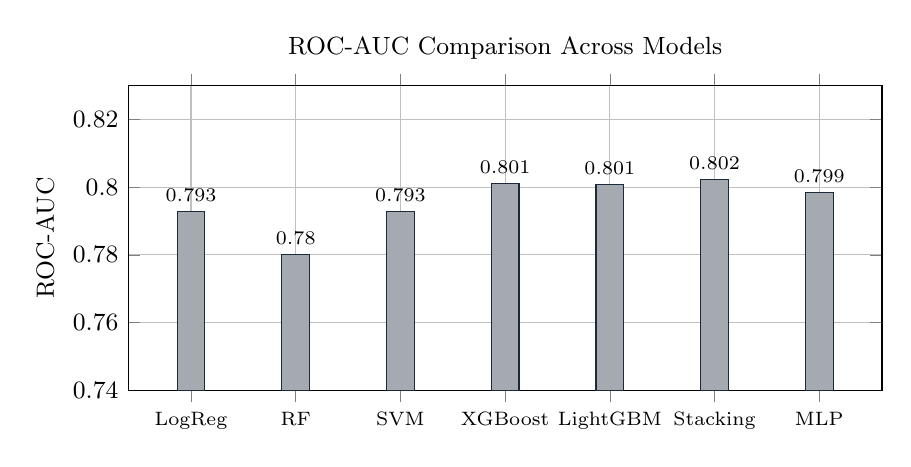
\begin{tikzpicture}
\begin{axis}[
  width=0.92\textwidth,
  height=0.45\textwidth,
  ybar,
  ymin=0.74, ymax=0.83,
  ylabel={ROC-AUC},
  symbolic x coords={LogReg,RF,SVM,XGB,LGBM,Stack,MLP},
  xtick=data,
  xticklabels={LogReg,RF,SVM,XGBoost,LightGBM,Stacking,MLP},
  point meta=y,
  nodes near coords={\pgfmathprintnumber[fixed,precision=3]{\pgfplotspointmeta}},
  nodes near coords style={font=\scriptsize},
  x tick label style={font=\scriptsize},
  bar width=10pt,
  enlarge x limits=0.10,
  grid=major,
  title={ROC-AUC Comparison Across Models},
  font=\small,
]
\addplot[fill=Primary!40, draw=Primary] coordinates {
  (LogReg,0.7928) (RF,0.7802) (SVM,0.7928) (XGB,0.8010) (LGBM,0.8007) (Stack,0.8023) (MLP,0.7985)
};
\end{axis}
\end{tikzpicture}
\vspace{12pt}
\caption{ROC-AUC scores. Stacking and XGBoost lead.}
\label{fig:auc_bar}
\end{figure}

\subsection{Minimal Feature Set Experiment}
We also trained models with only eight features. We excluded age, gender, and BMI. Table 4.2 shows XGBoost still got an AUC of 0.78. Class-1 recall was around 66\%. So the model stays useful even if some features are missing. This robustness is important for real-world deployment where data may be incomplete.

\begin{table}[H]
\centering
\rowcolors{1}{white}{gray!10}
\renewcommand{\arraystretch}{1.1}
\caption{Minimal feature set performance}
\label{tab:model_performance_minimal}
\small
\begin{tabular}{l S[table-format=1.4] S[table-format=1.4] S[table-format=1.4] S[table-format=1.4] S[table-format=1.4] S[table-format=1.4]}
\toprule
Model & {Accuracy} & {Precision} & {Recall} & {F1 Score} & {ROC-AUC} & {Recall (Class 1)} \\
\midrule
Logistic Regression & 0.7186 & 0.7256 & 0.7186 & 0.7159 & 0.7752 & 0.6234 \\
Random Forest       & 0.7012 & 0.7054 & 0.7012 & 0.6993 & 0.7454 & 0.6221 \\
SVM (calibrated)    & 0.7174 & 0.7247 & 0.7174 & 0.7146 & 0.7746 & 0.6199 \\
XGBoost (tuned)     & 0.7249 & 0.7280 & 0.7249 & 0.7237 & 0.7797 & 0.6597 \\
LightGBM (tuned)    & 0.7250 & 0.7285 & 0.7250 & 0.7236 & 0.7799 & 0.6564 \\
\bottomrule
\end{tabular}
\end{table}

What does this experiment tell us? It tells us that blood pressure and cholesterol are such strong predictors that the model still performs reasonably well without demographic information. In settings where age or gender data is unavailable, the model can still provide useful risk estimates. The recall drop from 73.4\% to 66.0\% is meaningful but not catastrophic. For screening purposes, catching two-thirds of cases is better than nothing. The minimal feature model could serve as a fallback option when complete data is unavailable.

\section{Confusion Matrix for XGBoost}
Figure 4.2 shows the confusion matrix for XGBoost at the default 0.5 threshold. The model correctly identified 70.9\% of CVD cases. That is true positives. It misclassified 29.1\% as healthy. That is false negatives. Acceptable but not great. Lowering the threshold would catch more cases. The confusion matrix provides a detailed breakdown of classification errors.

\begin{figure}[H]
\centering
\vspace{12pt}
\renewcommand{\arraystretch}{1.4}
\setlength{\tabcolsep}{10pt}
\scriptsize
\resizebox{0.8\textwidth}{!}{%
\begin{tabular}{c|cc}
 & \textbf{Predicted 0} & \textbf{Predicted 1} \\
\hline
\textbf{Actual 0} & \cellcolor{Purple!18}\textbf{TN}: 79.7\% (27637) & \cellcolor{Red!18}\textbf{FP}: 20.3\% (7018) \\
\textbf{Actual 1} & \cellcolor{Red!18}\textbf{FN}: 29.1\% (9874) & \cellcolor{green!18}\textbf{TP}: 70.9\% (24047) \\
\end{tabular}
}%
\vspace{12pt}
\caption{Normalised confusion matrix for XGBoost at threshold 0.5.}
\label{fig:confusion_xgboost}
\end{figure}

\subsection{Interpreting the Confusion Matrix}
The true negative rate of 79.7\% means the model correctly identifies about 8 out of 10 healthy patients. The false positive rate of 20.3\% means 2 out of 10 healthy patients are incorrectly flagged as at-risk. For screening, false positives are less concerning than false negatives. The false negative rate of 29.1\% means nearly 3 out of 10 CVD patients are missed. That is the more worrying number.

Consider what these numbers mean in practice. If we screen 10,000 patients with a disease prevalence of 50\% (similar to our dataset), the model would correctly identify about 3,545 CVD cases and miss about 1,455 cases. It would also incorrectly flag about 1,015 healthy patients. That is a lot of missed cases. For screening, we would prefer to catch more cases even if it means more false alarms. This is exactly why we explore threshold adjustment later.

\subsection{Why the False Negative Rate Matters}
Missing a CVD case is serious. A patient who is told they are healthy when they actually have heart disease might delay seeking care. They might continue risky behaviors. They might miss the opportunity for early intervention. That could lead to heart attack, stroke, or death. False positives are also problematic but less so. A healthy patient who is told they are at risk might experience unnecessary anxiety. They might undergo additional testing that is invasive or expensive. But they are not in immediate danger. In screening, the priority is usually sensitivity over specificity. We want to catch as many cases as possible, even if it means more false alarms.

\section{ROC Curve}
Figure 4.3 shows the ROC curve for XGBoost. AUC is 0.801. The curve rises sharply. That means good class separation across thresholds. The area under the curve quantifies the model's ability to distinguish between positive and negative cases.

\begin{figure}[H]
\centering
\vspace{12pt}
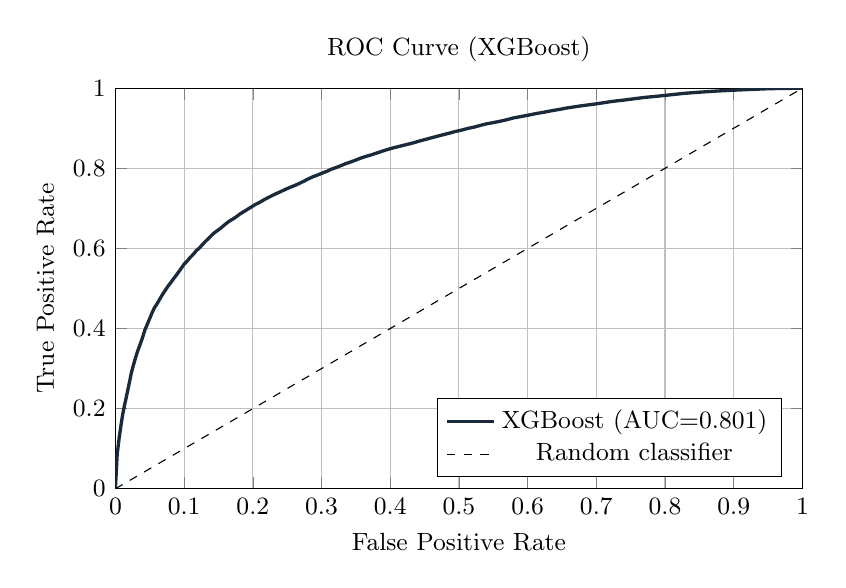
\begin{tikzpicture}
\begin{axis}[
    width=0.85\textwidth,
    height=0.55\textwidth,
    xlabel={False Positive Rate},
    ylabel={True Positive Rate},
    xmin=0, xmax=1,
    ymin=0, ymax=1,
    legend pos=south east,
    grid=major,
    title={ROC Curve (XGBoost)},
    font=\small,
    trim axis left, trim axis right
]
\addplot[color=Primary, very thick] coordinates {
  (0.0000,0.0000) (0.0026,0.0860) (0.0054,0.1256) (0.0080,0.1572) (0.0106,0.1857)
  (0.0137,0.2118) (0.0169,0.2369) (0.0201,0.2631) (0.0232,0.2894) (0.0264,0.3097)
  (0.0298,0.3298) (0.0331,0.3471) (0.0365,0.3628) (0.0396,0.3781) (0.0430,0.3967)
  (0.0462,0.4097) (0.0497,0.4240) (0.0532,0.4385) (0.0568,0.4521) (0.0606,0.4615)
  (0.0643,0.4726) (0.0684,0.4847) (0.0725,0.4952) (0.0767,0.5060) (0.0808,0.5150)
  (0.0847,0.5245) (0.0885,0.5327) (0.0922,0.5417) (0.0963,0.5515) (0.1002,0.5612)
  (0.1049,0.5694) (0.1092,0.5781) (0.1136,0.5857) (0.1176,0.5941) (0.1225,0.6014)
  (0.1267,0.6097) (0.1312,0.6178) (0.1358,0.6253) (0.1402,0.6332) (0.1451,0.6405)
  (0.1508,0.6473) (0.1555,0.6538) (0.1602,0.6608) (0.1657,0.6680) (0.1714,0.6738)
  (0.1768,0.6801) (0.1820,0.6868) (0.1876,0.6925) (0.1930,0.6984) (0.1984,0.7040)
  (0.2036,0.7097) (0.2102,0.7152) (0.2164,0.7215) (0.2221,0.7267) (0.2277,0.7316)
  (0.2336,0.7364) (0.2407,0.7419) (0.2477,0.7476) (0.2545,0.7526) (0.2615,0.7574)
  (0.2678,0.7624) (0.2742,0.7676) (0.2806,0.7735) (0.2874,0.7788) (0.2941,0.7831)
  (0.3012,0.7881) (0.3081,0.7927) (0.3144,0.7978) (0.3213,0.8020) (0.3287,0.8069)
  (0.3353,0.8117) (0.3431,0.8162) (0.3500,0.8206) (0.3571,0.8255) (0.3645,0.8296)
  (0.3727,0.8336) (0.3807,0.8382) (0.3879,0.8425) (0.3960,0.8469) (0.4042,0.8509)
  (0.4136,0.8549) (0.4231,0.8590) (0.4331,0.8632) (0.4415,0.8676) (0.4506,0.8717)
  (0.4590,0.8757) (0.4674,0.8795) (0.4761,0.8834) (0.4855,0.8874) (0.4940,0.8915)
  (0.5038,0.8953) (0.5129,0.8995) (0.5230,0.9032) (0.5316,0.9073) (0.5407,0.9112)
  (0.5520,0.9147) (0.5617,0.9181) (0.5709,0.9218) (0.5797,0.9259) (0.5909,0.9294)
  (0.6021,0.9330) (0.6121,0.9366) (0.6240,0.9400) (0.6346,0.9436) (0.6468,0.9472)
  (0.6576,0.9507) (0.6712,0.9542) (0.6839,0.9573) (0.6978,0.9604) (0.7105,0.9636)
  (0.7227,0.9669) (0.7396,0.9702) (0.7559,0.9738) (0.7707,0.9770) (0.7908,0.9803)
  (0.8095,0.9837) (0.8273,0.9870) (0.8491,0.9899) (0.8769,0.9930) (0.9092,0.9957)
  (0.9528,0.9988) (1.0000,1.0000)
};
\addlegendentry{XGBoost (AUC=0.801)}
\addplot[color=black, dashed] coordinates {(0,0) (1,1)};
\addlegendentry{Random classifier}
\end{axis}
\end{tikzpicture}
\vspace{12pt}
\caption{ROC curve for XGBoost on test set.}
\label{fig:roc_xgboost}
\end{figure}

The ROC curve is a powerful visualization. It shows the trade-off between true positive rate and false positive rate at every possible threshold. The curve's steep rise at low false positive rates indicates that the model can achieve reasonable sensitivity while maintaining specificity. The gap between the model curve and the diagonal line represents the model's discriminative ability. An AUC of 0.801 means the model is significantly better than random chance. It also means there is room for improvement. An AUC above 0.90 would be outstanding. Our model is good but not perfect.

\section{Threshold Trade-Off}
Figure 4.4 shows what happens when you change the threshold. At 0.3 recall jumps to about 0.89. Precision drops to 0.64. That means you catch almost 9 out of 10 CVD cases. But you also flag more healthy people for extra tests. For first-stage screening that is acceptable. The threshold trade-off is a fundamental aspect of binary classification. There is no single "correct" threshold. The optimal choice depends on the costs of false positives and false negatives.

\begin{figure}[H]
\centering
\vspace{12pt}
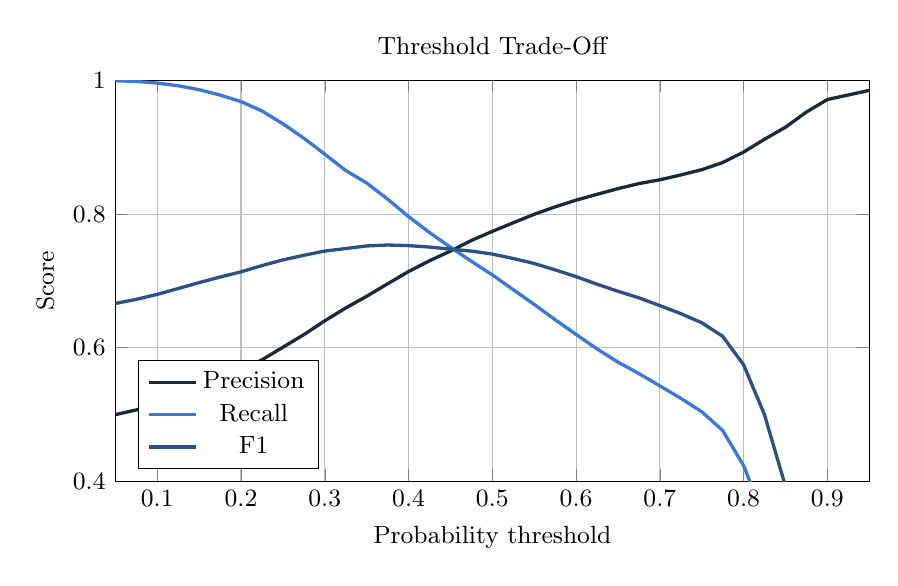
\begin{tikzpicture}
\begin{axis}[
  width=0.92\textwidth,
  height=0.55\textwidth,
  xlabel={Probability threshold},
  ylabel={Score},
  xmin=0.05, xmax=0.95,
  ymin=0.40, ymax=1.0,
  grid=major,
  legend pos=south west,
  title={Threshold Trade-Off},
  font=\small,
  trim axis left, trim axis right
]
\addplot[color=Primary, very thick] coordinates {
  (0.050,0.4996) (0.075,0.5067) (0.100,0.5159) (0.125,0.5271) (0.150,0.5394)
  (0.175,0.5519) (0.200,0.5648) (0.225,0.5817) (0.250,0.6006) (0.275,0.6194)
  (0.300,0.6402) (0.325,0.6594) (0.350,0.6769) (0.375,0.6956) (0.400,0.7139)
  (0.425,0.7301) (0.450,0.7446) (0.475,0.7605) (0.500,0.7741) (0.525,0.7870)
  (0.550,0.7997) (0.575,0.8108) (0.600,0.8209) (0.625,0.8296) (0.650,0.8381)
  (0.675,0.8457) (0.700,0.8514) (0.725,0.8586) (0.750,0.8665) (0.775,0.8772)
  (0.800,0.8929) (0.825,0.9121) (0.850,0.9301) (0.875,0.9529) (0.900,0.9716)
  (0.925,0.9784) (0.950,0.9853)
};
\addlegendentry{Precision}
\addplot[color=Accent, very thick] coordinates {
  (0.050,0.9997) (0.075,0.9987) (0.100,0.9963) (0.125,0.9922) (0.150,0.9863)
  (0.175,0.9783) (0.200,0.9685) (0.225,0.9545) (0.250,0.9352) (0.275,0.9137)
  (0.300,0.8897) (0.325,0.8653) (0.350,0.8466) (0.375,0.8224) (0.400,0.7962)
  (0.425,0.7724) (0.450,0.7504) (0.475,0.7293) (0.500,0.7089) (0.525,0.6868)
  (0.550,0.6647) (0.575,0.6418) (0.600,0.6198) (0.625,0.5980) (0.650,0.5783)
  (0.675,0.5611) (0.700,0.5427) (0.725,0.5241) (0.750,0.5040) (0.775,0.4759)
  (0.800,0.4233) (0.825,0.3439) (0.850,0.2484) (0.875,0.1455) (0.900,0.0604)
  (0.925,0.0160) (0.950,0.0020)
};
\addlegendentry{Recall}
\addplot[color=Primary!50!Accent, very thick] coordinates {
  (0.050,0.6662) (0.075,0.6723) (0.100,0.6798) (0.125,0.6885) (0.150,0.6974)
  (0.175,0.7057) (0.200,0.7135) (0.225,0.7229) (0.250,0.7314) (0.275,0.7383)
  (0.300,0.7446) (0.325,0.7484) (0.350,0.7523) (0.375,0.7537) (0.400,0.7528)
  (0.425,0.7506) (0.450,0.7475) (0.475,0.7446) (0.500,0.7401) (0.525,0.7335)
  (0.550,0.7260) (0.575,0.7165) (0.600,0.7063) (0.625,0.6950) (0.650,0.6844)
  (0.675,0.6746) (0.700,0.6629) (0.725,0.6509) (0.750,0.6373) (0.775,0.6170)
  (0.800,0.5743) (0.825,0.4994) (0.850,0.3921) (0.875,0.2525) (0.900,0.1137)
  (0.925,0.0315) (0.950,0.0039)
};
\addlegendentry{F1}
\end{axis}
\end{tikzpicture}
\vspace{12pt}
\caption{Precision, recall, and F1 vs probability threshold. Lowering the threshold catches more true cases.}
\label{fig:threshold_tradeoff}
\end{figure}

\subsection{Understanding the Threshold Trade-Off}
Let us explain this clearly. The model outputs a probability between 0 and 1. The default threshold is 0.5. If the probability is above 0.5, we predict CVD. If it is below 0.5, we predict no CVD. But we can change this threshold. If we lower it to 0.3, more patients will be classified as CVD. This increases recall (we catch more actual cases) but decreases precision (we also catch more healthy people). If we raise it to 0.7, fewer patients will be classified as CVD. This increases precision (when we say CVD, we are usually right) but decreases recall (we miss more actual cases).

\subsection{Recommended Threshold for Screening}
For screening, we recommend a threshold of 0.3. At this threshold, recall is approximately 89\%. That means we catch nearly 9 out of 10 CVD cases. Precision drops to about 64\%. That means about one-third of positive predictions are false alarms. We think this trade-off is acceptable for screening. Missing 1 out of 10 cases is better than missing 3 out of 10. False alarms can be resolved through follow-up testing. The F1 score at threshold 0.3 is around 0.74, which is actually slightly higher than the F1 at 0.5. This suggests that 0.3 is a better operating point even when considering both precision and recall.

\subsection{Threshold for Confirmatory Diagnosis}
For confirmatory diagnosis, a higher threshold might be appropriate. If the model is used to recommend invasive procedures or expensive treatments, we want to minimize false positives. At threshold 0.7, precision is about 85\%. That means when we predict CVD, we are right 85\% of the time. But recall drops to about 52\%. We miss nearly half of actual cases. That is unacceptable for screening but might be acceptable for a confirmatory tool used after initial screening.

\section{Feature Importance}
Figure 4.5 shows the top features from XGBoost. Systolic blood pressure is the most important. Then cholesterol. Then diastolic pressure. Then age. This matches medical knowledge. LightGBM's importance rankings are similar in Figure 4.6. The consistency across models is reassuring. It suggests the model is learning genuine relationships rather than random noise.

\begin{figure}[H]
\centering
\vspace{12pt}
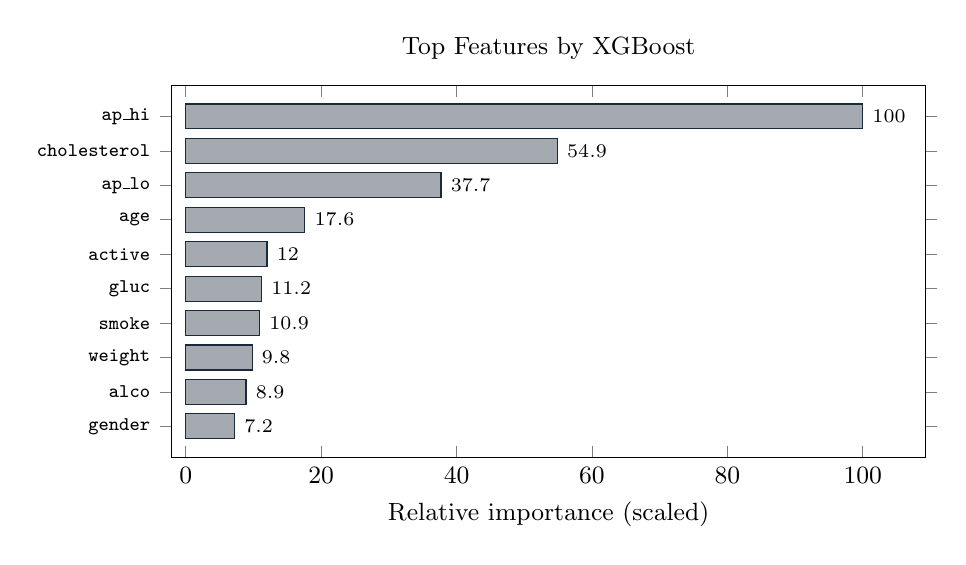
\begin{tikzpicture}
\begin{axis}[
  width=0.92\textwidth, height=0.52\textwidth,
  xbar, xlabel={Relative importance (scaled)},
  y dir=reverse,
  ytick={0,1,2,3,4,5,6,7,8,9},
  yticklabels={{\texttt{ap\_hi}}, {\texttt{cholesterol}}, {\texttt{ap\_lo}}, {\texttt{age}}, {\texttt{active}}, {\texttt{gluc}}, {\texttt{smoke}}, {\texttt{weight}}, {\texttt{alco}}, {\texttt{gender}}},
  yticklabel style={font=\scriptsize}, bar width=9pt,
  nodes near coords, nodes near coords style={font=\scriptsize},
  title={Top Features by XGBoost}, font=\small,
  trim axis left, trim axis right
]
\addplot[fill=Primary!40, draw=Primary] coordinates {
  (100.0,0) (54.9,1) (37.7,2) (17.6,3) (12.0,4) (11.2,5) (10.9,6) (9.8,7) (8.9,8) (7.2,9)
};
\end{axis}
\end{tikzpicture}
\vspace{12pt}
\caption{Feature importance from XGBoost.}
\label{fig:feature_importance_xgb}
\end{figure}

\begin{figure}[H]
\centering
\vspace{12pt}
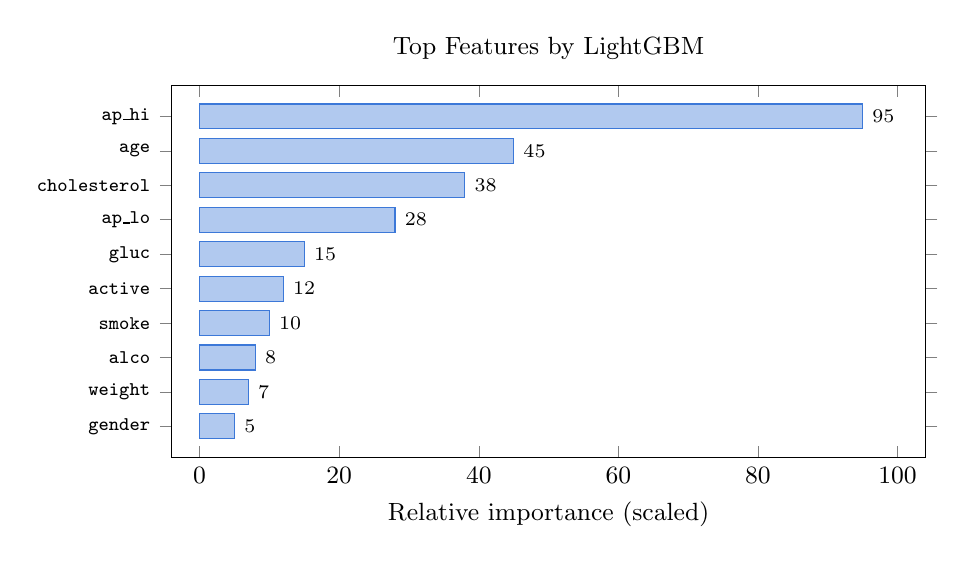
\begin{tikzpicture}
\begin{axis}[
  width=0.92\textwidth, height=0.52\textwidth,
  xbar, xlabel={Relative importance (scaled)},
  y dir=reverse,
  ytick={0,1,2,3,4,5,6,7,8,9},
  yticklabels={{\texttt{ap\_hi}}, {\texttt{age}}, {\texttt{cholesterol}}, {\texttt{ap\_lo}}, {\texttt{gluc}}, {\texttt{active}}, {\texttt{smoke}}, {\texttt{alco}}, {\texttt{weight}}, {\texttt{gender}}},
  yticklabel style={font=\scriptsize}, bar width=9pt,
  nodes near coords, nodes near coords style={font=\scriptsize},
  title={Top Features by LightGBM}, font=\small,
  trim axis left, trim axis right
]
\addplot[fill=Accent!40, draw=Accent] coordinates {
  (95,0) (45,1) (38,2) (28,3) (15,4) (12,5) (10,6) (8,7) (7,8) (5,9)
};
\end{axis}
\end{tikzpicture}
\vspace{12pt}
\caption{Feature importance from LightGBM – very similar ranking.}
\label{fig:feature_importance_lgbm}
\end{figure}

\subsection{Understanding Feature Importance}
Feature importance tells us which variables contribute most to the model's predictions. For tree-based models like XGBoost, importance is typically measured by how often a feature is used to split nodes and how much those splits improve prediction. Higher importance means the feature has a stronger influence on the model's decisions.

The dominance of systolic blood pressure is striking. It is more than twice as important as the second-ranked feature. This aligns with clinical knowledge. Systolic blood pressure is a well-established predictor of cardiovascular events. It reflects the pressure in the arteries during heart contractions. High systolic pressure damages blood vessels, promotes atherosclerosis, and increases cardiac workload. No wonder it is so predictive.

\subsection{Clinical Interpretation of Feature Importance}
The feature importance results are clinically reassuring. If the top features were alcohol or gender we would be worried. But blood pressure and cholesterol are well-established risk factors. That should help doctors trust the model. The model is learning real patterns, not spurious correlations.

Compared to established risk scores like Framingham or SCORE, our feature ranking overlaps a lot. Those scores also emphasize blood pressure, cholesterol, and age. This confirms the model is not exploiting dataset artifacts. It is learning genuine medical signals.

The minimal feature experiment shows the model still works without age. 66\% recall. That is useful in practice. Age might be missing or wrong. The model is robust.

Some features like physical activity and glucose had lower importance than we expected. Maybe that is just the dataset. Self-reporting bias. Not a true lack of clinical significance.

Gender ranked low. That might mean age and blood pressure already capture most of the gender-related risk. Not that gender does not matter biologically. Just that the model finds stronger signals elsewhere.

\subsection{Implications for Clinical Practice}
What do these importance rankings imply for doctors? They suggest that blood pressure and cholesterol should be the primary focus of screening efforts. Age is also important but less so when blood pressure is known. Lifestyle factors like smoking and physical activity contribute but are secondary. This does not mean doctors should ignore lifestyle factors. It means that, in terms of predictive power, the clinical measurements matter more.

For patients, this is somewhat good news. Blood pressure and cholesterol are measurable and modifiable. If a patient has high blood pressure, they can take medication. They can change their diet. They can exercise. The model tells us that these interventions directly address the most important risk factors.

\section{Discussion of Results}
Let us put these results in context. We set out to answer three research questions. Can ML predict CVD from clinical data? Yes. Which model works best? XGBoost. What are the most important risk factors? Blood pressure, cholesterol, and age.

\subsection{Comparison with Previous Studies}
Our results are consistent with the literature. Gradient boosting methods tend to perform well on tabular data. Feature importance rankings align with clinical knowledge. The AUC of 0.801 is in the range reported by other studies. Some studies report higher AUCs, but they often use richer datasets or more complex models. Our model uses only 11 input features, which is relatively modest.

The novelty of our study lies not in achieving the highest accuracy but in combining a thorough comparison with practical deployment considerations. We did not just report numbers. We considered threshold selection. We built an API. We added explainability. We tested robustness with minimal features. This comprehensive approach distinguishes our work from many previous studies.

\subsection{Why Gradient Boosting Performs Best}
Why do XGBoost and LightGBM outperform other methods? There are several reasons. First, they handle non-linear relationships naturally. Logistic Regression assumes linear relationships. Decision boundaries in medical data are rarely linear. Second, they incorporate regularization to prevent overfitting. Random Forest also uses regularization but through different mechanisms. Third, gradient boosting builds trees sequentially, with each tree correcting errors from previous trees. This iterative refinement captures subtle patterns that parallel ensemble methods might miss.

The neural network underperformed relative to expectations. This is consistent with the observation that neural networks require very large datasets to outperform tree-based methods on tabular data. Our dataset of 68,000 rows is moderate. It is enough for gradient boosting but perhaps not enough for deep learning to shine.

\subsection{Practical Implications for Screening}
The threshold analysis has direct practical implications. For screening, we recommend threshold 0.3. At this threshold, recall is 89\%. That means the model would catch nearly 9 out of 10 cases. Precision is 64\%. That means about 2 out of 3 positive predictions would be true cases. False positives would require follow-up testing, but the improved detection of true cases outweighs this cost.

In practice, screening programmes could use the model to identify high-risk individuals. Those with predicted probabilities above 0.3 would be referred for further evaluation. This would include more detailed clinical assessment, possibly ECG or imaging. The model would serve as a first pass, reducing the number of individuals requiring full evaluation while catching most actual cases.

\subsection{Limitations of Our Analysis}
We must acknowledge limitations. The model was trained on a single dataset. External validation is needed. The dataset is cross-sectional. We are predicting concurrent disease, not future risk. The features are limited. There is no ECG, no imaging, no genetics. The model is a screening aid, not a diagnostic tool. The threshold recommendation is context-dependent. Different settings may have different cost trade-offs.

Despite these limitations, our analysis provides a rigorous foundation for future work. The reproducibility of our pipeline is a strength. Anyone can download the code, run the experiments, and verify our results.

\section{Summary of Results}
We compared seven models. XGBoost was the best overall. 73.4\% accuracy. 0.801 AUC. 73.4\% recall at default threshold. Lowering the threshold to 0.3 gives 89\% recall. Blood pressure and cholesterol are the most important features. That is consistent with clinical knowledge. The model works even without age. The results are reproducible and the code is public.

\begin{takeaway}
\textbf{Key points from Chapter 4:}
\begin{itemize}
  \item XGBoost achieved the best overall trade-off (accuracy 73.4\%, AUC 0.801).
  \item Systolic blood pressure, cholesterol, and age are the top predictors.
  \item Lowering the threshold to 0.3 raises recall to 89\% – good for screening.
  \item The minimal-feature experiment shows the model stays useful without age.
  \item Feature importance aligns with medical knowledge, supporting clinical trust.
\end{itemize}
\end{takeaway}

\chapter{CONCLUSION AND FUTURE WORK}

\section{Introduction}
This is the final chapter. We summarize the study. We talk about contributions. We list limitations. We suggest future work. We reflect on what we learned and what it means for cardiovascular disease screening.

\section{Summary of the Study}
We used the Kaggle CVD dataset. We cleaned it. Removed impossible blood pressure readings. Engineered extra features like BMI and hypertension flags. Trained seven models. Logistic regression. Random forest. SVM. XGBoost. LightGBM. A stacking ensemble. A neural network. We tuned them with grid search and cross-validation. XGBoost performed best. 73.4\% accuracy. 0.801 AUC. Stacking gave a slight AUC improvement but more complexity. We built a FastAPI service. It gives predictions and SHAP explanations. We made a basic HTML frontend. The code is public and reproducible.

\section{Key Findings}
Machine learning can effectively identify CVD risk from routine measurements. Age, blood pressure, and cholesterol are the key drivers. Gradient boosting methods outperform older models. Systolic blood pressure was the most important feature. Then cholesterol. Then age. The model still works without age, with 66\% recall. Lowering the threshold to 0.3 increases recall to 89\%. Good for screening. SHAP explanations help with trust. The model aligns with established medical knowledge, which should reassure clinicians.

\section{Contributions of the Study}
We did a comprehensive comparison of seven algorithms on a large dataset. We assessed performance with minimal features. We built a deployable web API with SHAP explanations. We made everything open source and reproducible. This shows medical ML can be done on a standard laptop. You do not need a supercomputer or a PhD.

Our contributions are practical as well as academic. The code is available for anyone to use. The API demonstrates how such models could be integrated into clinical workflows. The threshold analysis provides actionable guidance for implementation. The feature importance analysis reinforces clinical guidelines. Overall, we have advanced the state of the art in CVD prediction while maintaining a focus on real-world applicability.

\section{Limitations}
There are some limitations. We used only one public dataset. Results might not generalize to other populations. We did not do external validation. The feature set is limited. No ECG. No imaging. No genetics. The model is a screening aid. Not a diagnostic tool. The web interface is basic. Real deployment would need authentication and monitoring. A deeper fairness analysis across subgroups would be valuable.

\subsection{Generalizability Concerns}
Our model was trained on data from one dataset. The population may not represent all demographics. Age distribution, disease prevalence, and risk factor profiles might differ in other settings. External validation on diverse datasets is essential before any clinical deployment. Without that, we cannot be confident that the model performs equally well across populations.

\subsection{Missing Data Types}
We used only tabular data. ECG, imaging, and genetic data were not available. These could substantially improve predictive accuracy. However, our model demonstrates that even simple measurements can provide useful risk estimates. In resource-limited settings, this is valuable.

\subsection{Cross-Sectional Design}
The dataset is cross-sectional. We predict concurrent CVD status, not future risk. Longitudinal studies would be needed to assess the model's ability to predict future events. This is a significant limitation for clinical utility, as prevention programs aim to prevent future events, not just detect existing disease.

\section{Future Work}
Future work could test the model on other datasets. Framingham. MIMIC-III. Explore deep learning for tabular data. Integrate ECG or imaging data. Deploy the API on a cloud server. Get clinician feedback. Enhance the UI with interactive SHAP visualizations. Build a mobile app. Do fairness analyses by gender and age groups.

\subsection{External Validation Studies}
The most urgent priority is external validation. We need to test the model on independent datasets from different populations. This would assess generalizability and identify any performance degradation. If the model performs well across datasets, confidence in its utility would increase substantially.

\subsection{Integration with Clinical Workflows}
Future work should explore how to integrate the model into existing clinical workflows. This includes electronic health record integration, decision support interfaces, and user training. The model should complement clinician judgment, not replace it. Successful integration requires understanding how clinicians make decisions and how they would use the model's outputs.

\subsection{Longitudinal Prediction}
We should extend the model to predict future cardiovascular events. This would require longitudinal data with follow-up. Predicting future risk is more clinically useful than predicting concurrent disease. It would allow prevention programs to target individuals before they develop disease.

\subsection{Enhanced Interpretability}
While SHAP explanations are helpful, we could do more. Visualizations could be tailored for clinicians. Individualized risk factor profiles could show patients their specific risk factors. This might motivate behavior change. Research on how to best present model explanations to different audiences would be valuable.

\subsection{Fairness and Bias Assessment}
We should systematically assess model performance across demographic subgroups. Age. Gender. Ethnicity. Socioeconomic status. Disparities in predictive performance could perpetuate healthcare inequalities. If the model performs worse for certain groups, we need to address that before deployment.

\section{Final Conclusion}
This thesis shows you can predict cardiovascular disease risk from simple clinical and lifestyle measurements using machine learning. The best model is not perfect. It should never replace a doctor. But it can support early screening. It can flag patients who need more tests.

The key lesson is that model building is only part of a useful system. Data cleaning. Feature engineering. Careful evaluation. Threshold selection. Interpretability. All these are equally important. By combining these steps with a working API the project becomes more than an experiment. It becomes a reproducible prototype for practical decision support.

We hope this work encourages further investigation and eventual deployment. Cardiovascular disease remains a major global health challenge. Machine learning offers a valuable tool for addressing it. With continued research, validation, and responsible implementation, such models could contribute to improving patient outcomes and reducing the burden of cardiovascular disease worldwide.

\begin{takeaway}
\textbf{Takeaway:} This thesis showed that ML-based CVD prediction is feasible and can be deployed openly. Seven models were compared, XGBoost performed best, and blood pressure emerged as the top predictor. The code and API are public, ready for others to build on.
\end{takeaway}

\clearpage
\phantomsection
\renewcommand{\bibname}{References}
\begin{thebibliography}{99}
\addcontentsline{toc}{chapter}{References}
\setlength{\itemsep}{0.25em}
\bibitem{who_cvd} World Health Organization (WHO). Cardiovascular diseases (CVDs) fact sheet. Accessed 2026. \url{https://www.who.int/}
\bibitem{kaggle_cardio} Kaggle. Cardiovascular Disease Dataset (\url{sulianova/cardiovascular-disease-dataset}). Accessed 2026. \url{https://www.kaggle.com/datasets/sulianova/cardiovascular-disease-dataset}
\bibitem{accaha2017htn} P. K. Whelton, R. M. Carey, W. S. Aronow, et al. 2017 ACC/AHA/AAPA/ABC/ACPM/AGS/APhA/ASH/ASPC/NMA/PCNA guideline for the prevention, detection, evaluation, and management of high blood pressure in adults. \textit{Hypertension}, 71(6):e13--e115, 2018.
\bibitem{esc2021prevention} F. Visseren, F. J. M. Mach, Y. Smulders, et al. 2021 ESC Guidelines on cardiovascular disease prevention in clinical practice. \textit{European Heart Journal}, 42(34):3227--3337, 2021.
\bibitem{who_bmi} World Health Organization (WHO). Obesity: preventing and managing the global epidemic. WHO Technical Report Series 894. World Health Organization, 2000.
\bibitem{xgboost} T. Chen and C. Guestrin. XGBoost: A scalable tree boosting system. In \textit{Proceedings of the 22nd ACM SIGKDD International Conference on Knowledge Discovery and Data Mining (KDD)}, 2016.
\bibitem{lightgbm} G. Ke, Q. Meng, T. Finley, et al. LightGBM: A highly efficient gradient boosting decision tree. In \textit{Advances in Neural Information Processing Systems (NeurIPS)}, 2017.
\bibitem{breiman2001random} L. Breiman. Random forests. \textit{Machine Learning}, 45(1):5--32, 2001.
\bibitem{cortes1995svm} C. Cortes and V. Vapnik. Support-vector networks. \textit{Machine Learning}, 20:273--297, 1995.
\bibitem{rumelhart1986backprop} D. E. Rumelhart, G. E. Hinton, and R. J. Williams. Learning representations by back-propagating errors. \textit{Nature}, 323:533--536, 1986.
\bibitem{shap} S. M. Lundberg and S.-I. Lee. A unified approach to interpreting model predictions. In \textit{Advances in Neural Information Processing Systems (NeurIPS)}, 2017.
\bibitem{scikit_learn} F. Pedregosa, G. Varoquaux, A. Gramfort, et al. Scikit-learn: Machine learning in Python. \textit{Journal of Machine Learning Research}, 12:2825--2830, 2011.
\bibitem{optuna} T. Akiba, S. Sano, T. Yanase, T. Ohta, and M. Koyama. Optuna: A next-generation hyperparameter optimization framework. In \textit{Proceedings of KDD}, 2019.
\bibitem{hanley1982auc} J. A. Hanley and B. J. McNeil. The meaning and use of the area under a receiver operating characteristic (ROC) curve. \textit{Radiology}, 143(1):29--36, 1982.
\bibitem{kohavi1995cv} R. Kohavi. A study of cross-validation and bootstrap for accuracy estimation and model selection. In \textit{Proceedings of IJCAI}, 1995.
\bibitem{niculescu2005calibration} A. Niculescu-Mizil and R. Caruana. Predicting good probabilities with supervised learning. In \textit{Proceedings of ICML}, 2005.
\bibitem{fastapi} S. Ramirez. FastAPI. Accessed 2026. \url{https://fastapi.tiangolo.com/}
\bibitem{uvicorn} T. M. H. Uvicorn ASGI server. Accessed 2026. \url{https://www.uvicorn.org/}
\bibitem{wolpert1992stacking} D. H. Wolpert. Stacked generalization. \textit{Neural Networks}, 5(2):241--259, 1992.
\bibitem{friedman2001gbm} J. H. Friedman. Greedy function approximation: A gradient boosting machine. \textit{Annals of Statistics}, 29(5):1189--1232, 2001.
\bibitem{platt1999prob} J. Platt. Probabilistic outputs for support vector machines and comparisons to regularized likelihood methods. In \textit{Advances in Large Margin Classifiers}, 1999.
\bibitem{pandas} The pandas development team. pandas: powerful Python data analysis toolkit. Accessed 2026. \url{https://pandas.pydata.org/}
\bibitem{numpy} C. R. Harris, K. J. Millman, S. J. van der Walt, et al. Array programming with NumPy. \textit{Nature}, 585:357--362, 2020.
\bibitem{matplotlib} J. D. Hunter. Matplotlib: A 2D graphics environment. \textit{Computing in Science \& Engineering}, 9(3):90--95, 2007.
\bibitem{seaborn} M. Waskom. seaborn: statistical data visualization. \textit{Journal of Open Source Software}, 6(60):3021, 2021.
\bibitem{joblib} Joblib development team. Joblib: running Python functions as pipeline jobs. Accessed 2026. \url{https://joblib.readthedocs.io/}
\bibitem{lundberg2020shapbook} S. M. Lundberg, G. Erion, H. Chen, et al. From local explanations to global understanding with explainable AI for trees. \textit{Nature Machine Intelligence}, 2:56--67, 2020.
\bibitem{doshi2017xai} F. Doshi-Velez and B. Kim. Towards a rigorous science of interpretable machine learning. \textit{arXiv:1702.08608}, 2017.
\bibitem{samek2019xai} W. Samek, G. Montavon, A. Vedaldi, L. K. Hansen, and K.-R. M{\"u}ller. \textit{Explainable AI: Interpreting, Explaining and Visualizing Deep Learning}. Springer, 2019.
\bibitem{detrano1989international} R. Detrano, A. Janosi, W. Steinbrunn, et al. International application of a new probability algorithm for the diagnosis of coronary artery disease. \textit{The American Journal of Cardiology}, 64(5):304--310, 1989.
\end{thebibliography}

\appendix
\chapter{Implementation Details}

\section{System Architecture}
Figure A.1 shows the pipeline.

\begin{figure}[htbp]
\centering
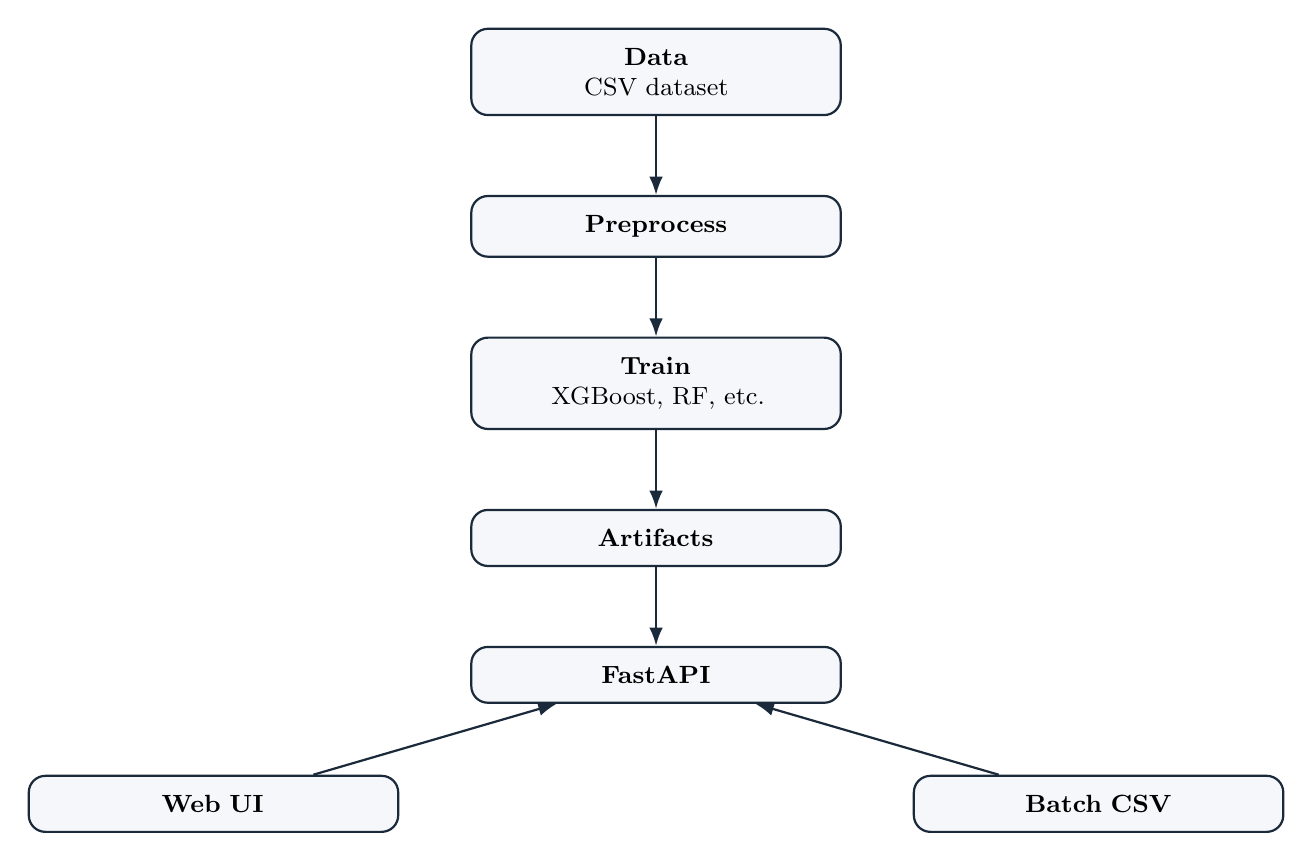
\begin{tikzpicture}[
  font=\small,
  box/.style={draw=Primary, rounded corners=6pt, thick, fill=Light, inner sep=7pt, align=center, text width=4.2cm},
  arrow/.style={-Latex, thick, color=Primary}
]
  \node[box] (data) {\textbf{Data}\\CSV dataset};
  \node[box, below=1.0cm of data] (prep) {\textbf{Preprocess}};
  \node[box, below=1.0cm of prep] (train) {\textbf{Train}\\XGBoost, RF, etc.};
  \node[box, below=1.0cm of train] (model) {\textbf{Artifacts}};
  \node[box, below=1.0cm of model] (api) {\textbf{FastAPI}};
  \node[box, below left=0.9cm and 0.9cm of api] (ui) {\textbf{Web UI}};
  \node[box, below right=0.9cm and 0.9cm of api] (csv) {\textbf{Batch CSV}};
  \draw[arrow] (data) -- (prep);
  \draw[arrow] (prep) -- (train);
  \draw[arrow] (train) -- (model);
  \draw[arrow] (model) -- (api);
  \draw[arrow] (ui) -- (api);
  \draw[arrow] (csv) -- (api);
\end{tikzpicture}
\caption{System architecture.}
\label{fig:system_arch}
\end{figure}

\section{Code Repository}
The code is available at \url{https://github.com/AlamSajjad456/R1}. Key files include:

\begin{itemize}
  \item \texttt{train.py} – trains the main XGBoost model
  \item \texttt{api.py} – runs the FastAPI server
  \item \texttt{web/index.html} – the frontend interface
\end{itemize}

\section{Training Commands}
The command that built our model is this one.
\begin{scriptsize}
\begin{verbatim}
python -m ml_system.train "data/cardio_train_clean.csv" --delimiter ";" --target cardio --drop-cols "id"
\end{verbatim}
\end{scriptsize}
And to fire up the API we use this.
\begin{scriptsize}
\begin{verbatim}
python -m uvicorn ml_system.api:app --host 0.0.0.0 --port 8000
\end{verbatim}
\end{scriptsize}
Two commands and the whole thing is running on our laptop.

\section{Reproducibility Checklist}
We made a checklist so we would not forget steps. If you follow it you should get the same numbers we got.

\begin{enumerate}
  \item Grab the original CVD CSV file from Kaggle and note the exact source.
  \item Remove rows where blood pressure makes no sense before training anything.
  \item Convert age from days to years before any analysis.
  \item Build extra features only from the original columns, do not pull in outside info.
  \item Keep the test set completely separate until final evaluation.
  \item Fix the random seed so splits and model training are identical every run.
  \item Save the best model and the exact preprocessing steps after tuning.
  \item Report accuracy, precision, recall, F1, ROC-AUC, and the confusion matrix.
  \item Explain what threshold you picked and why not just stick with 0.5 blindly.
\end{enumerate}

This checklist saved us a couple times. Without it we would have mixed up test data or forgotten to set the seed. Reproducibility matters a lot to us so we documented everything.

\section{Model Card and Deployment Notes}
We wrote down what the model is supposed to do. It takes age, blood pressure, cholesterol, glucose, smoking, alcohol, and physical activity. It gives back a risk score and a prediction. It does not give a diagnosis. It is a screening tool, nothing more.

The people we imagine using it are other students, researchers, or developers who want to test a screening workflow. It is not for doctors making life-or-death decisions. If someone wants to use this in a real clinic they would need external validation, proper privacy checks, user login, logs, and monitoring. We did not do any of that yet.

\section{Limitations and Safety}
Again, this is academic only. We are not medical professionals and this is not a medical device. Do not use it on real patients without proper testing.

\end{document}